\documentclass[11pt, a4paper, logo, copyright, nonumbering]{deepmind}
\usepackage[authoryear, sort&compress, round]{natbib}
\usepackage{dblfloatfix}
\usepackage{ulem}
\usepackage{caption}
\usepackage{subcaption}
\usepackage{listings}
\lstset{breaklines=true}
\usepackage{longtable}
\usepackage{dramatist}
\usepackage{xspace}
\usepackage{pifont}% http://ctan.org/pkg/pifont
\usepackage{multirow}
\usepackage{tcolorbox}
\usepackage{xltabular}
\usepackage{longtable}
\usepackage{hyperref}
\interfootnotelinepenalty=10000

\usepackage{amsfonts}
\usepackage{amsmath}
\usepackage{amssymb}
\usepackage{lineno}

\usepackage[bottom]{footmisc}

% 中文支持 - 必须在加载其他宏包后设置
\usepackage{fontspec}
\usepackage{xeCJK}
% 设置CJK字体
\setCJKmainfont[AutoFakeBold=true,AutoFakeSlant=true]{STSong}
\setCJKsansfont[AutoFakeBold=true]{STHeiti}
\setCJKmonofont{STFangsong}
% 强制所有CJK字符使用CJK字体  
\xeCJKsetup{CJKmath=false, PlainEquation=true}

\makeatletter
\def\@BTrule[#1]{%
  \ifx\longtable\undefined
    \let\@BTswitch\@BTnormal
  \else\ifx\hline\LT@hline
    \nobreak
    \let\@BTswitch\@BLTrule
  \else
     \let\@BTswitch\@BTnormal
  \fi\fi
  \global\@thisrulewidth=#1\relax
  \ifnum\@thisruleclass=\tw@\vskip\@aboverulesep\else
  \ifnum\@lastruleclass=\z@\vskip\@aboverulesep\else
  \ifnum\@lastruleclass=\@ne\vskip\doublerulesep\fi\fi\fi
  \@BTswitch}
\makeatother

\addto\extrasenglish{
    \def\chapterautorefname{Chapter}%
    \def\sectionautorefname{Section}%
    \def\subsectionautorefname{Section}
    \def\subsubsectionautorefname{Section}
    \def\paragraphautorefname{Paragraph}%
    \def\tableautorefname{Table}%
    \def\equationautorefname{Equation}%
}

\newenvironment{indentchunk}[1]%
 {\begin{list}{}%
         {\setlength{\leftmargin}{#1}}%
         \item[]%
 }
 {\end{list}}
 
\bibliographystyle{abbrvnat}

\newcommand{\massivetext}{\textit{MassiveText}\xspace}
\newcommand{\massiveweb}{\textit{MassiveWeb}\xspace}

\newcommand{\gopher}{\textit{Gopher}\xspace}
\newcommand{\nummodels}{400 }
\newcommand{\Gopher}{\textit{Gopher}\xspace}
\newcommand{\chinchilla}{\textit{Chinchilla}\xspace}
\newcommand{\Chinchilla}{\textit{Chinchilla}\xspace}
\newcommand{\mtnlg}{MT-NLG 530B\xspace}
\newcommand{\bigbench}{BIG-bench\xspace}
\newcommand{\gopherchat}{\textit{Dialogue-Prompted Gopher}\xspace}
\newcommand{\gopherchatsl}{\textit{Dialogue-Tuned Gopher}\xspace}
\newcommand{\perspectiveapi}{\textit{Perspective API}\xspace}
\newcommand{\user}{\textit{User}\xspace}
\newcommand{\cmark}{\ding{51}}%
\newcommand{\xmark}{\ding{55}}%
\newcommand{\tcotwoe}{tCO\textsubscript{2}e\xspace}
\newcommand{\pygithub}{\texttt{python\_github}\xspace}

\correspondingauthor{email@email}

\reportnumber{001}

\renewcommand{\today}{}

\title{\centering 训练计算最优的大型语言模型}

\correspondingauthor{ \{jordanhoffmann|sborgeaud|amensch|sifre\}@deepmind.com}

\author[$\star$]{Jordan~Hoffmann}
\author[$\star$]{Sebastian~Borgeaud}
\author[$\star$]{Arthur~Mensch}

\author[  \hspace{-.8ex}]{Elena~Buchatskaya}
\author[  \hspace{-.8ex}]{Trevor~Cai}
\author[  \hspace{-.8ex}]{Eliza~Rutherford}
\author[  \hspace{-.8ex}]{Diego~de~Las~Casas}
\author[  \hspace{-.8ex}]{Lisa~Anne~Hendricks}
\author[  \hspace{-.8ex}]{Johannes~Welbl}
\author[  \hspace{-.8ex}]{Aidan~Clark}
\author[  \hspace{-.8ex}]{Tom~Hennigan}
\author[  \hspace{-.8ex}]{Eric~Noland}
\author[  \hspace{-.8ex}]{Katie~Millican}
\author[  \hspace{-.8ex}]{George~van~den~Driessche}
\author[  \hspace{-.8ex}]{Bogdan~Damoc}
\author[  \hspace{-.8ex}]{Aurelia~Guy}
\author[  \hspace{-.8ex}]{Simon~Osindero}
\author[  \hspace{-.8ex}]{Karen~Simonyan}
\author[  \hspace{-.8ex}]{Erich~Elsen}
\author[  \hspace{-.8ex}]{Jack~W.~Rae}
\author[  \hspace{-.8ex}]{Oriol~Vinyals}
\author[$\star$]{Laurent~Sifre}

\affil[$\star$]{同等贡献}

\usepackage[titles]{tocloft}
\setlength{\cftbeforesecskip}{-.5ex}

\renewcommand\cftsubsecfont{\small}
\renewcommand\cftsubsecpagefont{\small}

\input{commands.tex}

\begin{abstract}
我们研究了在给定计算预算下训练Transformer语言模型的最优模型规模和Token数量。
我们发现当前的大型语言模型存在明显的训练不足问题,这是近期在扩大语言模型规模时保持训练数据量不变的结果。
通过训练超过\nummodels个参数规模从7000万到超过160亿的语言模型,在50亿到5000亿Token上进行训练,我们发现对于计算最优的训练,模型规模和训练Token数量应该等比例缩放:每当模型规模翻倍时,训练Token数量也应该翻倍。
我们通过训练一个预测的计算最优模型\chinchilla来测试这一假设,该模型使用与\gopher相同的计算预算,但只有70B参数和4倍的数据量。
\chinchilla在大量下游评估任务上全面且显著地优于\Gopher (280B)、GPT-3 (175B)、Jurassic-1 (178B)和Megatron-Turing NLG (530B)。
这也意味着\chinchilla在微调和推理时使用的计算量大大减少,极大地便利了下游应用。
值得强调的是,\chinchilla在MMLU基准测试上达到了67.5\%的最先进平均准确率,比\gopher提高了超过7\%。
\end{abstract}

\begin{document}

% 重新应用CJK字体设置
\setCJKmainfont[AutoFakeBold=true,AutoFakeSlant=true]{STSong}
\setCJKsansfont[AutoFakeBold=true]{STHeiti}
\setCJKmonofont{STFangsong}

\maketitle

\section{引言}
最近推出了一系列\textit{大型语言模型} (LLMs) \citep{gpt3, jurassic, rae2021gopher, nlg530b, thoppilan2022lamda},目前最大的密集语言模型已经拥有超过5000亿参数。
这些大型自回归Transformer \citep{vaswani2017attention}在使用各种评估协议(如零样本、少样本和微调)的许多任务上展现了令人印象深刻的性能。

训练大型语言模型的计算和能源成本是巨大的 \citep{rae2021gopher, thoppilan2022lamda},并且随着模型规模的增加而上升。
在实践中,分配的训练计算预算通常是预先知道的:有多少加速器可用以及我们想使用它们多长时间。
由于通常只能训练这些大型模型一次,因此准确估计给定计算预算下的最佳模型超参数至关重要 \citep{tay2021scale}。

\citet{kaplan2020scaling}表明,自回归语言模型(LM)中的参数数量与其性能之间存在幂律关系。
因此,该领域一直在训练越来越大的模型,期待性能改进。
\citet{kaplan2020scaling}的一个值得注意的结论是,大型模型不应该被训练到其可能的最低损失才是计算最优的。
虽然我们得出了相同的结论,但我们估计大型模型应该接受比作者建议的更多训练Token的训练。
具体而言,给定$10\times$的计算预算增加,他们建议模型规模应增加$5.5\times$,而训练Token数量应仅增加1.8$\times$。
相反,我们发现模型规模和训练Token数量应该以相等的比例缩放。

遵循\citet{kaplan2020scaling}和GPT-3的训练设置 \citep{gpt3},许多最近训练的大型模型都在大约3000亿Token上进行训练(\autoref{tab:llms}),这与在增加计算量时主要增加模型规模的方法一致。

\begin{figure*}[t]
    \centering
    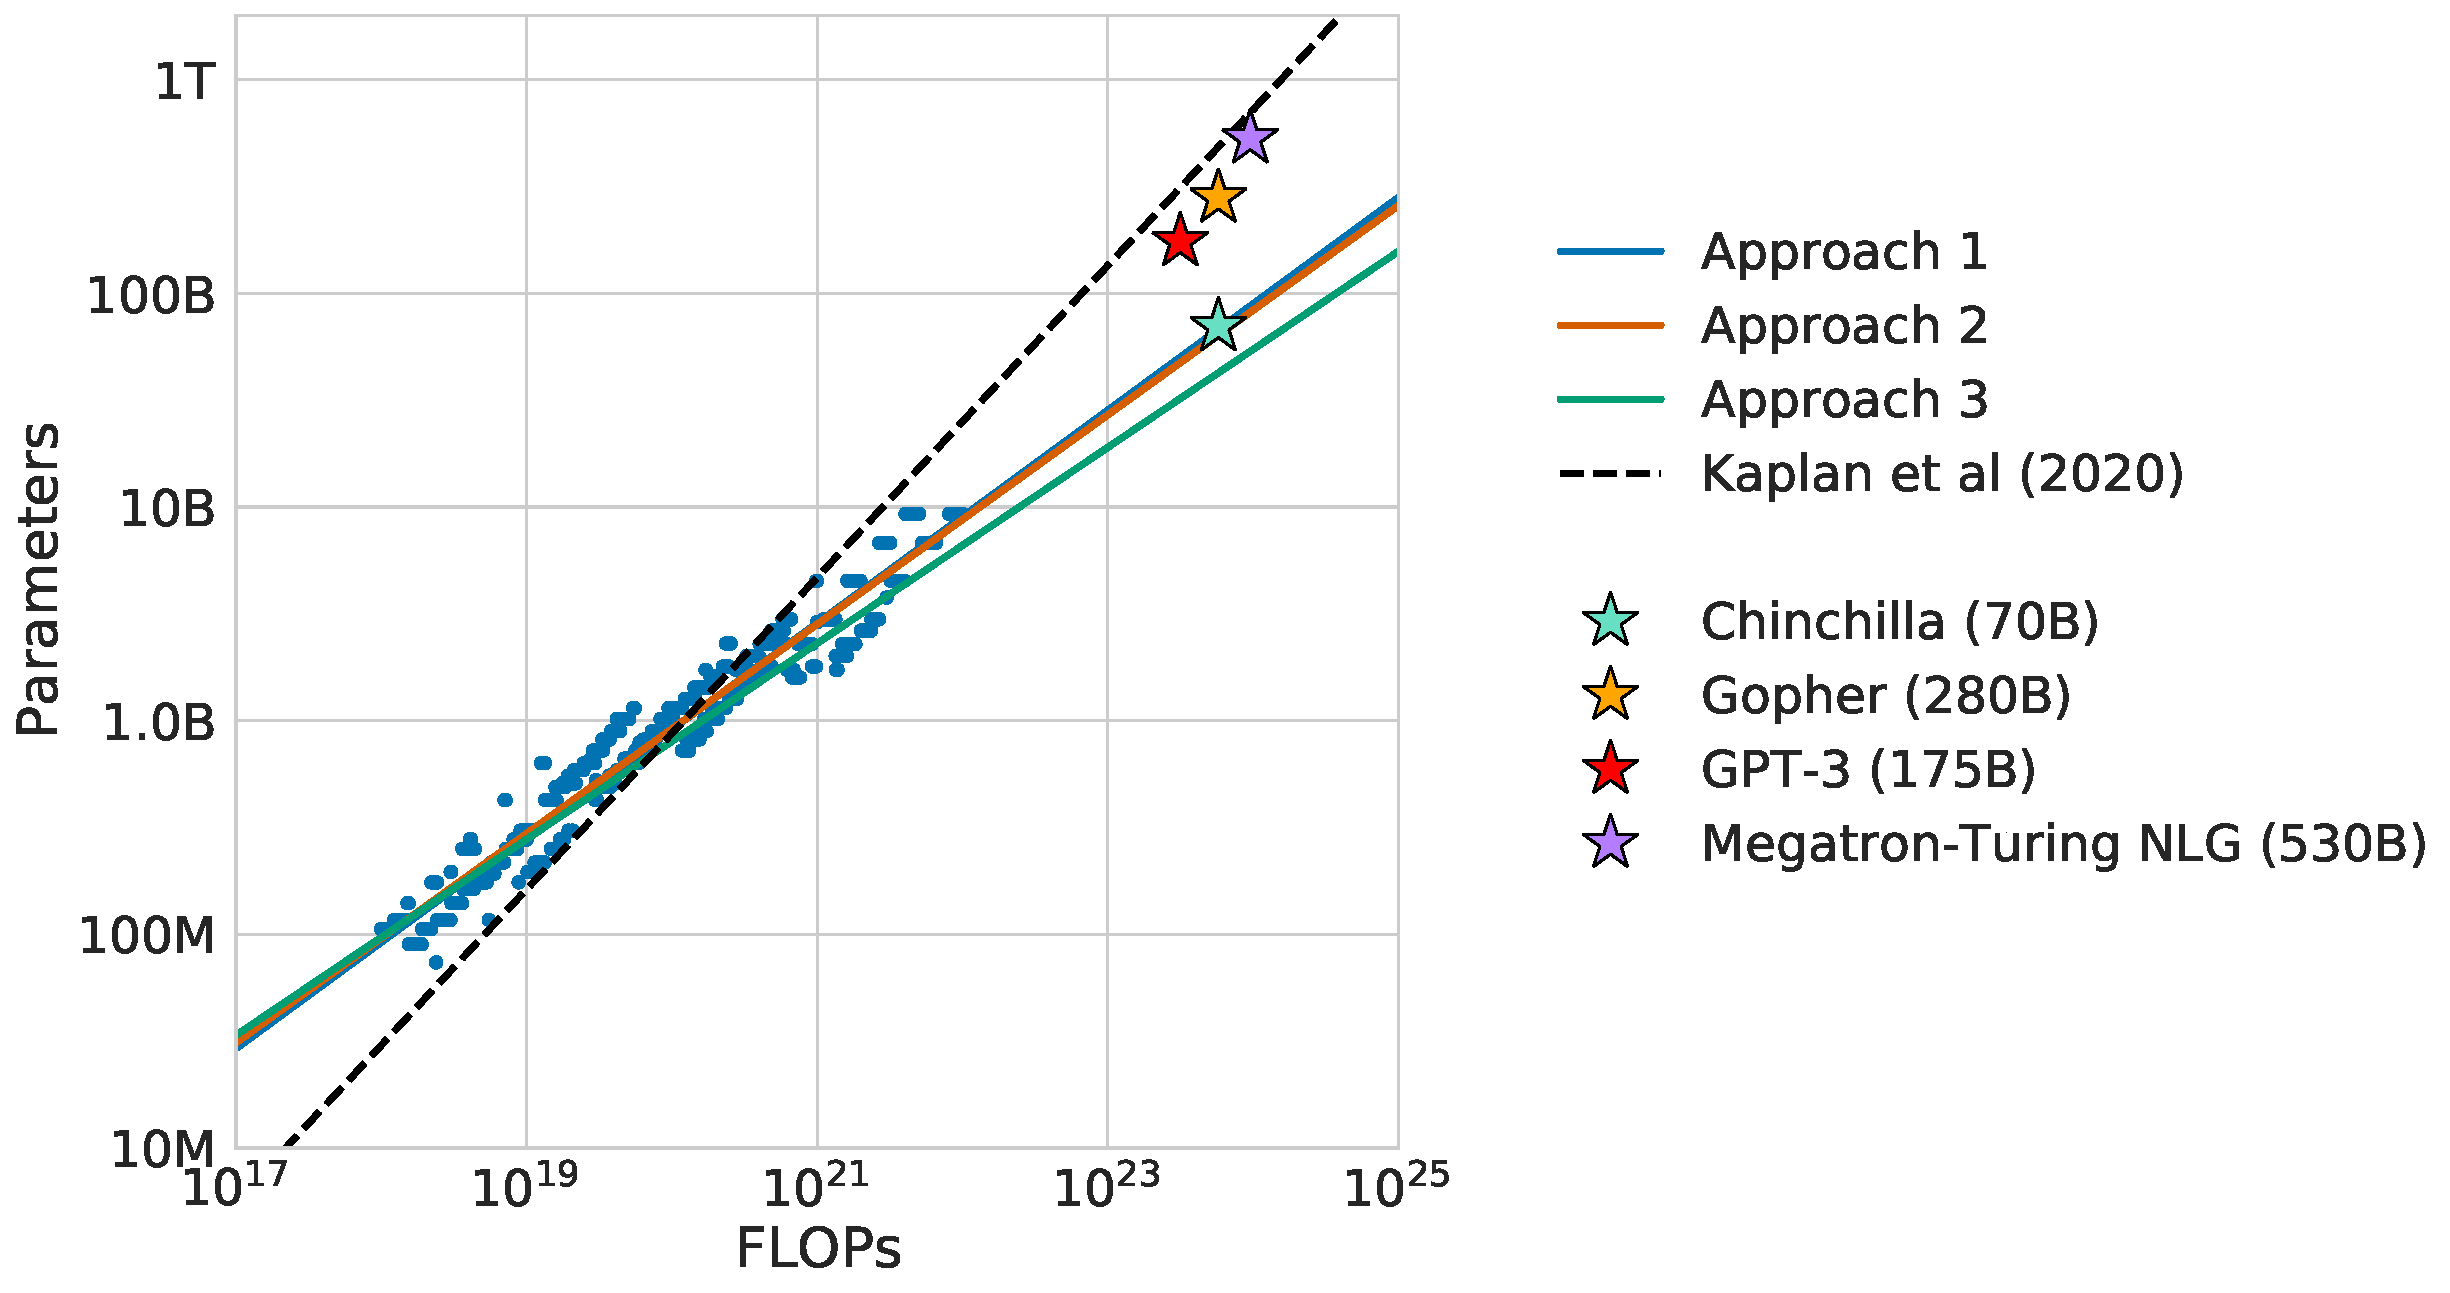
\includegraphics[width=.9\textwidth, trim=-5cm 0 0 0]{figures/combined_predictions_v9.pdf}
    \caption{\textbf{叠加预测。}
    我们将三种不同方法的预测与\citet{kaplan2020scaling}的预测一起叠加显示。我们发现所有三种方法都预测当前的大型模型应该更小得多,因此训练时间应该更长。
    在\autoref{fig:token_flop}中,我们显示了针对固定FLOP预算的最优Token数量与最优参数数量的关系。
    \textbf{\chinchilla优于\gopher和其他大型模型(见\autoref{sec:model_analysis})。}
    }
    \label{fig:combined_predictions}
\end{figure*}

\begin{table*}[t]
    \caption{\textbf{当前的大型语言模型。}
    我们展示了当前五个最大的密集Transformer模型、它们的规模和训练Token数量。除了LaMDA \citep{thoppilan2022lamda}之外,大多数模型都在大约3000亿Token上进行训练。
    我们引入了\chinchilla,一个规模更小的模型,训练时间远超过300B Token。
    }
    \label{tab:llms}
\centering
\begin{tabular}{l r c}
\toprule
模型 & 规模 (参数数量) & 训练Token数 \\
\midrule
LaMDA \citep{thoppilan2022lamda} & 1370亿 & 1680亿 \\
GPT-3 \citep{gpt3} & 1750亿 & 3000亿 \\
Jurassic \citep{jurassic} & 1780亿 & 3000亿 \\
\gopher \citep{rae2021gopher} & 2800亿 & 3000亿 \\
\mtnlg \citep{nlg530b} & 5300亿 & 2700亿\\
\midrule
\chinchilla & 700亿 & 1.4万亿\\
\bottomrule
\end{tabular}
\end{table*}

在本工作中,我们重新审视这个问题:
\textit{给定固定的FLOPs预算,\footnote{例如,知道加速器的数量和目标训练持续时间。}应该如何权衡模型规模和训练Token数量?}
为了回答这个问题,我们将最终的预训练损失\footnote{
为简单起见,我们对平滑的训练损失进行分析,这是测试损失的无偏估计,因为我们处于无限数据范围(训练Token数量少于整个语料库中的Token数量)。}
$L(N, D)$建模为模型参数数量~$N$和训练Token数量~$D$的函数。
由于计算预算$C$是已见训练Token数量和模型参数的确定性函数$\text{FLOPs}(N,D)$,我们关心在约束$\text{FLOPs}(N, D) = C$下最小化$L$:
% 
\begin{equation}\label{eq:model}
    N_{opt}(C), D_{opt}(C) = \argmin_{N, D \text{ s.t. } \text{FLOPs}(N, D) = C} L(N, D).
\end{equation}
% 
函数$N_{opt}(C)$和$D_{opt}(C)$描述了计算预算$C$的最优分配。
我们基于超过\nummodels个模型的损失来经验估计这些函数,这些模型的参数范围从不到$70$M到超过$16$B,在$5$B到超过$400$B Token上进行训练——每个模型配置都针对几个不同的训练周期进行训练。
我们的方法得出了与\citet{kaplan2020scaling}大不相同的结果。
我们在\autoref{fig:combined_predictions}中突出显示我们的结果,在\autoref{sec:related_work}中说明我们的方法如何不同。

基于我们估计的计算最优前沿,我们预测对于用于训练\gopher的计算预算,最优模型应该小4倍,同时在4倍的Token上进行训练。
我们通过训练一个更\textit{计算最优}的70B模型\chinchilla来验证这一点,该模型在1.4万亿Token上进行训练。
\chinchilla不仅优于其更大的对应模型\gopher,而且其减小的模型规模大大降低了推理成本,并极大地便利了在较小硬件上的下游使用。
大型语言模型的能源成本通过其用于推理和微调的使用来分摊。
因此,更优训练的较小模型的好处不仅限于其改进性能的直接好处。

\section{相关工作}
\label{sec:related_work}
\paragraph{大型语言模型。}
过去几年引入了各种大型语言模型。
这些包括密集Transformer模型 \citep{gpt3, jurassic, nlg530b, rae2021gopher, thoppilan2022lamda}和混合专家(MoE)模型 \citep{du2021glam, fedus2021switch, zoph2022designing}。
最大的密集Transformer已经超过5000亿参数 \citep{nlg530b}。
训练越来越大的模型的动力是明确的——到目前为止,增加语言模型的规模一直负责改进许多语言建模任务的最先进水平。
尽管如此,大型语言模型面临几个挑战,包括它们巨大的计算需求(训练和推理成本随模型规模增加) \citep{rae2021gopher, thoppilan2022lamda}以及获取更多高质量训练数据的需求。
事实上,在本工作中我们发现更大、更高质量的数据集将在语言模型的任何进一步扩展中发挥关键作用。

\paragraph{建模缩放行为。}
理解语言模型的缩放行为及其迁移特性对于近期大型模型的发展很重要 \citep{kaplan2020scaling,  hernandez2021scaling}。
\citet{kaplan2020scaling}首次展示了模型规模和损失之间在许多数量级上的可预测关系。
作者研究了为给定计算预算选择最优模型规模的问题。与我们类似,他们通过训练各种模型来解决这个问题。
我们的工作在几个重要方面与\citet{kaplan2020scaling}不同。
首先,作者对所有模型使用固定数量的训练Token和学习率调度;这阻止了他们建模这些超参数对损失的影响。
相比之下,我们发现将学习率调度设置为大致匹配训练Token数量可以获得最佳的最终损失,无论模型规模如何——见\autoref{fig:cosine}。
对于固定到130B Token的学习率余弦调度,中间损失估计(对于$D' << 130$B)因此高估了使用与$D'$匹配的调度长度训练的模型的损失。
使用这些中间损失会导致低估在少于130B Token数据上训练模型的有效性,并最终导致模型规模应该比训练数据规模增长更快的结论(随着计算预算的增加)。
相比之下,我们的分析预测这两个量应该以大致相同的速率缩放。
其次,我们包括了高达16B参数的模型,因为我们观察到FLOP-损失前沿存在轻微曲率(见\autoref{app:curvature})——事实上,我们分析中使用的大多数模型都有超过5亿参数,相比之下\citet{kaplan2020scaling}中的大多数运行要小得多——许多少于1亿参数。

最近,\citet{clark2022unified}专门研究了混合专家语言模型的缩放属性,表明随着模型规模的增加,专家数量的缩放效果会减弱——他们的方法将损失建模为两个变量的函数:模型规模和专家数量。
然而,分析是在固定数量的训练Token下完成的,与\citet{kaplan2020scaling}一样,可能低估了分支的改进。

\paragraph{估计大型模型的超参数。}
在选择语言模型和训练程序时,模型规模和训练Token数量不是唯一需要选择的两个参数。
其他重要因素包括学习率、学习率调度、批量大小、优化器和宽度-深度比。
在本工作中,我们专注于模型规模和训练步数,并依赖现有工作和提供的实验启发式方法来确定其他必要的超参数。
\citet{yang2021tuning}研究了如何为训练自回归Transformer选择各种这些参数,包括学习率和批量大小。
\citet{mccandlish2018empirical}发现最优批量大小和模型规模之间只有微弱的依赖关系。\citet{shallue2018measuring, NEURIPS2019_e0eacd98}建议使用比我们使用的更大的批量大小是可能的。
\citet{levine2020depth}研究了各种标准模型规模的最优深度-宽度比。我们使用的模型稍微不那么深,因为这在我们的硬件上转化为更好的实时性能。

\paragraph{改进的模型架构。}
最近,提出了各种有前途的传统密集Transformer替代方案。
例如,通过使用条件计算,大型MoE模型如1.7万亿参数的Switch Transformer \citep{fedus2021switch}、1.2万亿参数的GLaM模型 \citep{du2021glam}和其他模型 \citep{artetxe2021efficient, zoph2022designing}能够提供大的有效模型规模,尽管使用相对较少的训练和推理FLOP。
然而,对于非常大的模型,路由模型的计算优势似乎会减弱 \citep{clark2022unified}。
改进语言模型的一个正交方法是用显式检索机制增强Transformer,如\citet{borgeaud2021retrieval, guu2020realm, lewisretrieval2020}所做的。这种方法有效地增加了训练期间看到的数据Token数量(在\citet{borgeaud2021retrieval}中增加了约$\sim10$倍)。
这表明语言模型的性能可能比以前认为的更依赖于训练数据的规模。

\section{估计最优参数/训练Token分配}
\label{sec:method}
我们提出三种不同的方法来回答驱动我们研究的问题:
\textit{给定固定的FLOPs预算,应该如何权衡模型规模和训练Token数量?}
在所有三种情况下,我们首先训练一系列模型,改变模型规模和训练Token数量,并使用得到的训练曲线来拟合它们应该如何缩放的经验估计器。
我们假设计算和模型规模之间存在幂律关系,正如\citet{clark2022unified, kaplan2020scaling}中所做的那样,尽管未来的工作可能希望在大模型规模下包括这种关系中的潜在曲率。
所有三种方法的结果预测相似,并表明参数计数和训练Token数量应该随着更多计算而平等增加\footnote{我们如\autoref{sec:flops}中所述计算FLOP。}——比例在\autoref{tab:comparison}中报告。
这与之前关于这个主题的工作形成鲜明对比,值得进一步研究。

\subsection{方法1:固定模型规模并改变训练Token数量}

在我们的第一种方法中,我们为固定的模型家族(范围从70M到超过10B参数)改变训练步数,每个模型针对4种不同数量的训练序列进行训练。
从这些运行中,我们能够直接提取对于给定数量的训练FLOP所达到的最小损失的估计。此方法的训练细节可在\autoref{sec:scaling_details}中找到。

\begin{figure*}[t]
    \centering
    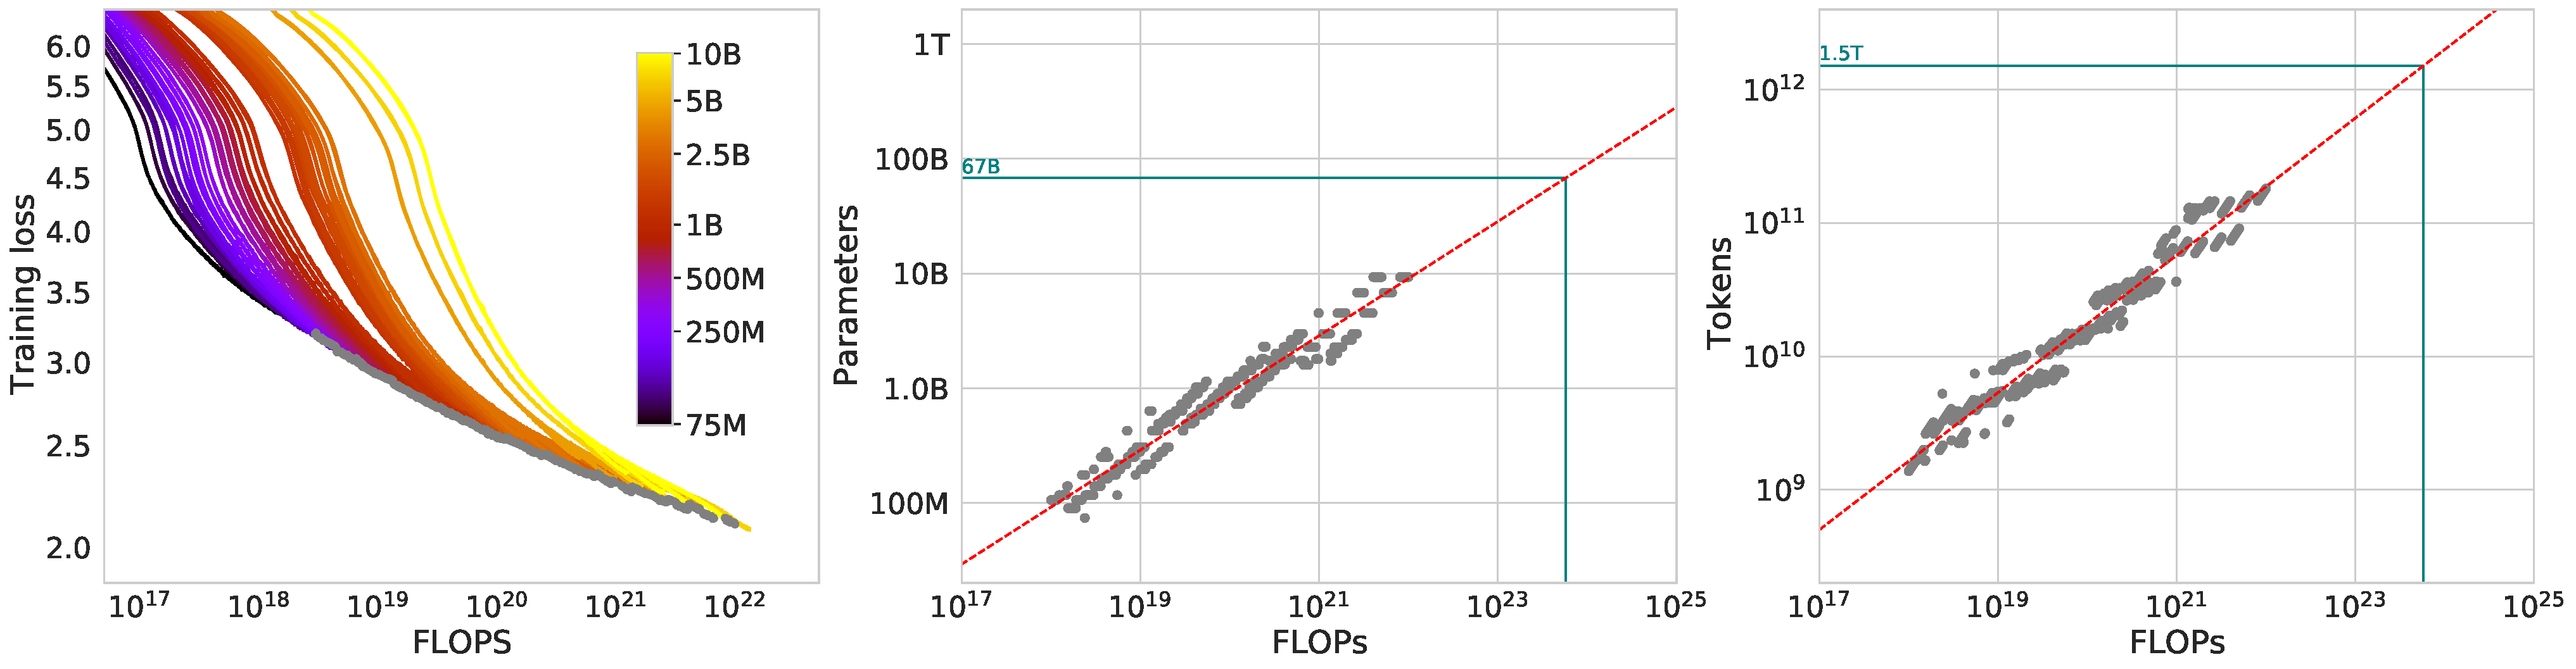
\includegraphics[width=.95\textwidth]{figures/scaling_11.pdf}
    \caption{\textbf{训练曲线包络。}在\textbf{左侧}我们显示所有不同的运行。我们启动了一系列模型规模,从70M到10B,每个都有四种不同的余弦周期长度。从这些曲线中,我们提取了每个FLOP的最小损失包络,并使用这些点来估计给定计算预算的最优模型规模(\textbf{中心})和最优训练Token数量(\textbf{右侧})。
    在绿色中,我们显示了基于用于训练\gopher的FLOP数量($5.76 \times 10^{23}$)的最优模型规模和训练Token数量预测。
    }
    \label{fig:approach1}
\end{figure*}

对于每个参数计数$N$,我们训练4个不同的模型,在一个范围(以训练Token数量衡量)上将学习率衰减$10\times$倍,该范围相差$16 \times$倍。
然后,对于每次运行,我们平滑然后插值训练损失曲线。
由此,我们获得从FLOP计数到每次运行的训练损失的连续映射。
然后,对于每个FLOP计数,我们确定哪次运行达到最低损失。
使用这些插值,我们获得从任何FLOP计数$C$到模型规模$N$和训练Token数量$D$的最有效选择的映射,使得$\text{FLOPs}(N,D) = C$。\footnote{注意所有选定的点都在训练的最后15\%内。这表明当在$D$ Token上训练模型时,我们应该选择一个余弦周期长度,在大约$D$ Token上衰减$10 \times$——见\autoref{sec:cosine_cycle}中的更多细节。}
在1500个对数间隔的FLOP值处,我们找到哪个模型规模在所有模型中达到最低损失以及所需的训练Token数量。
最后,我们拟合幂律来估计任何给定计算量的最优模型规模和训练Token数量(见\autoref{fig:approach1}的中心和右侧面板),获得关系$N_{opt} \propto C^a$和$D_{opt} \propto C^b$。
我们发现$a=0.50$和$b=0.50$——如\autoref{tab:comparison}中总结的那样。
在\autoref{app:kaplan_comparison}中,我们展示了在$10^{21}$FLOP下的直接比较,使用我们的分析推荐的模型规模和\citet{kaplan2020scaling}的分析——使用我们预测的模型规模有明显优势。

\subsection{方法2:IsoFLOP曲线}
在我们的第二种方法中,我们为固定的9个不同训练FLOP计数集合\footnote{训练Token数量由模型规模和训练FLOP确定。}(范围从$6 \times10^{18}$到$3 \times 10^{21}$FLOP)改变模型规模\footnote{在方法2中,模型规模变化高达16B,而在方法1中我们只使用了高达10B的模型。},并考虑每个点的最终训练损失\footnote{我们将余弦调度长度设置为匹配Token数量,根据\autoref{sec:cosine_cycle}中呈现的分析这是最优的。},与方法1考虑整个训练运行中的点$(N, D, L)$形成对比。
这使我们能够直接回答问题:对于给定的FLOP预算,最优参数计数是多少?

对于每个FLOP预算,我们在\autoref{fig:isoflop}(左)中绘制最终损失(平滑后)与参数计数的关系。
在所有情况下,我们确保训练了足够多样化的模型规模集合以看到损失的明确最小值。
我们对每条IsoFLOP曲线拟合抛物线以直接估计在什么模型规模下达到最小损失(\autoref{fig:isoflop}(左))。
与之前的方法一样,我们然后在FLOP和损失最优模型规模以及训练Token数量之间拟合幂律,如\autoref{fig:isoflop}(中心,右侧)所示。
再次,我们拟合形式为$N_{opt} \propto C^a$和$D_{opt} \propto C^b$的指数,我们发现$a=0.49$和$b=0.51$——如\autoref{tab:comparison}中总结的那样。

\begin{figure*}[t]
    \centering
    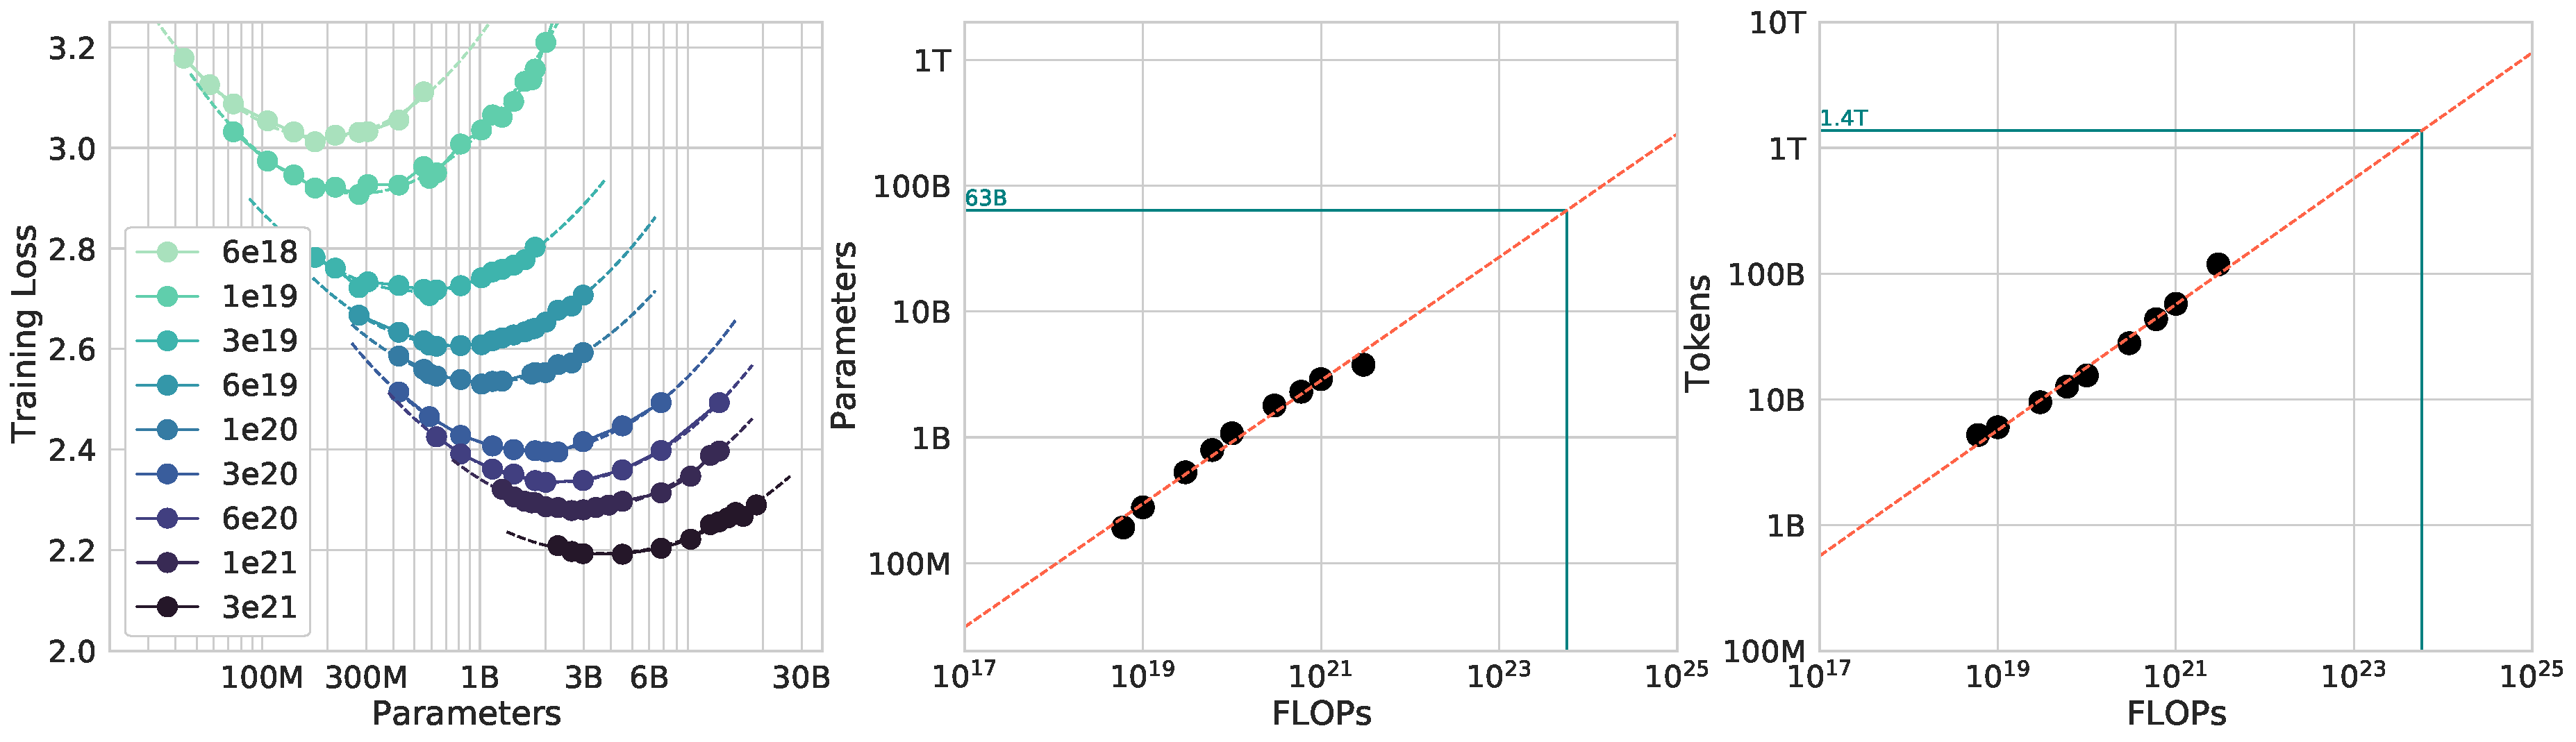
\includegraphics[width=.95\textwidth]{figures/isoflop_7.pdf}
    \caption{\textbf{IsoFLOP曲线。}对于各种模型规模,我们选择训练Token数量使得最终FLOP是一个常数。余弦周期长度设置为匹配目标FLOP计数。我们发现损失中存在明确的谷值,意味着对于给定的FLOP预算存在一个最优模型(\textbf{左})。
    使用这些谷值的位置,我们预测更大模型的最优模型规模和Token数量(\textbf{中心}和\textbf{右})。
    在绿色中,我们显示了使用\gopher的计算预算训练的\textit{最优}模型的估计参数数量和Token数量。
    }
    \label{fig:isoflop}
\end{figure*}

\subsection{方法3:拟合参数化损失函数}
最后,我们将方法1和2中实验的所有最终损失建模为模型参数计数和已见Token数量的参数化函数。
遵循经典风险分解(见\autoref{sec:approach3}),我们提出以下函数形式
\begin{equation}
    \hat L(N,D) \triangleq E + \frac{A}{N^\alpha} + \frac{B}{D^\beta}.\label{eq:decompose}
\end{equation}
第一项捕获数据分布上理想生成过程的损失,应该对应于自然文本的熵。
第二项捕获具有$N$个参数的完美训练Transformer表现不及理想生成过程的事实。
最后一项捕获Transformer没有训练到收敛的事实,因为我们只在数据集分布的样本上进行有限数量的优化步骤。

\paragraph{模型拟合。}为了估计$(A, B, E, \alpha, \beta)$,我们使用L-BFGS算法 \citep{nocedal_updating_1980}最小化预测和观察到的对数损失之间的Huber损失 \citep{huber_robust_1964}:
\begin{align}
    \min_{A, B, E, \alpha, \beta}\quad &\sum_{\text{运行 }i} \text{Huber}_\delta \Big(\log \hat L(N_i, D_i) - \log L_i\Big) \label{eq:huber}
\end{align}
我们通过从初始化网格中选择最佳拟合来考虑可能的局部最小值。
Huber损失($\delta=10^{-3}$)对异常值具有鲁棒性,我们发现这对于在保留数据点上的良好预测性能很重要。\autoref{app:parametric}详细说明了拟合过程和损失分解。

\paragraph{高效前沿。}
我们可以通过在约束$\text{FLOPs}(N, D) \approx 6 N D$ \citep{kaplan2020scaling}下最小化参数化损失$\hat L$来近似函数$N_{opt}$和$D_{opt}$。
得到的$N_{opt}$和$D_{opt}$平衡方程~\eqref{eq:huber}中依赖于模型规模和数据的两项。
通过构造,它们具有幂律形式:
\begin{equation}
    N_{opt}(C) = G {\left(\frac{C}{6}\right)}^{a}, \quad
    D_{opt}(C) = G^{-1} {\left(\frac{C}{6}\right)}^{b}, \quad \text{其中 }\quad
    G = {\left(\frac{\alpha A}{\beta B} \right)}^{\frac{1}{\alpha + \beta}},\quad
    a = \frac{\beta}{\alpha+\beta}, \text{且} b = \frac{\alpha}{\alpha + \beta}.
\end{equation}
我们在\autoref{fig:approach_3}(左)中显示拟合函数$\hat L$的等高线,以及蓝色的闭式高效计算前沿。
从这种方法,我们发现$a=0.46$和$b=0.54$——如\autoref{tab:comparison}中总结的那样。

\begin{figure}
    \centering
    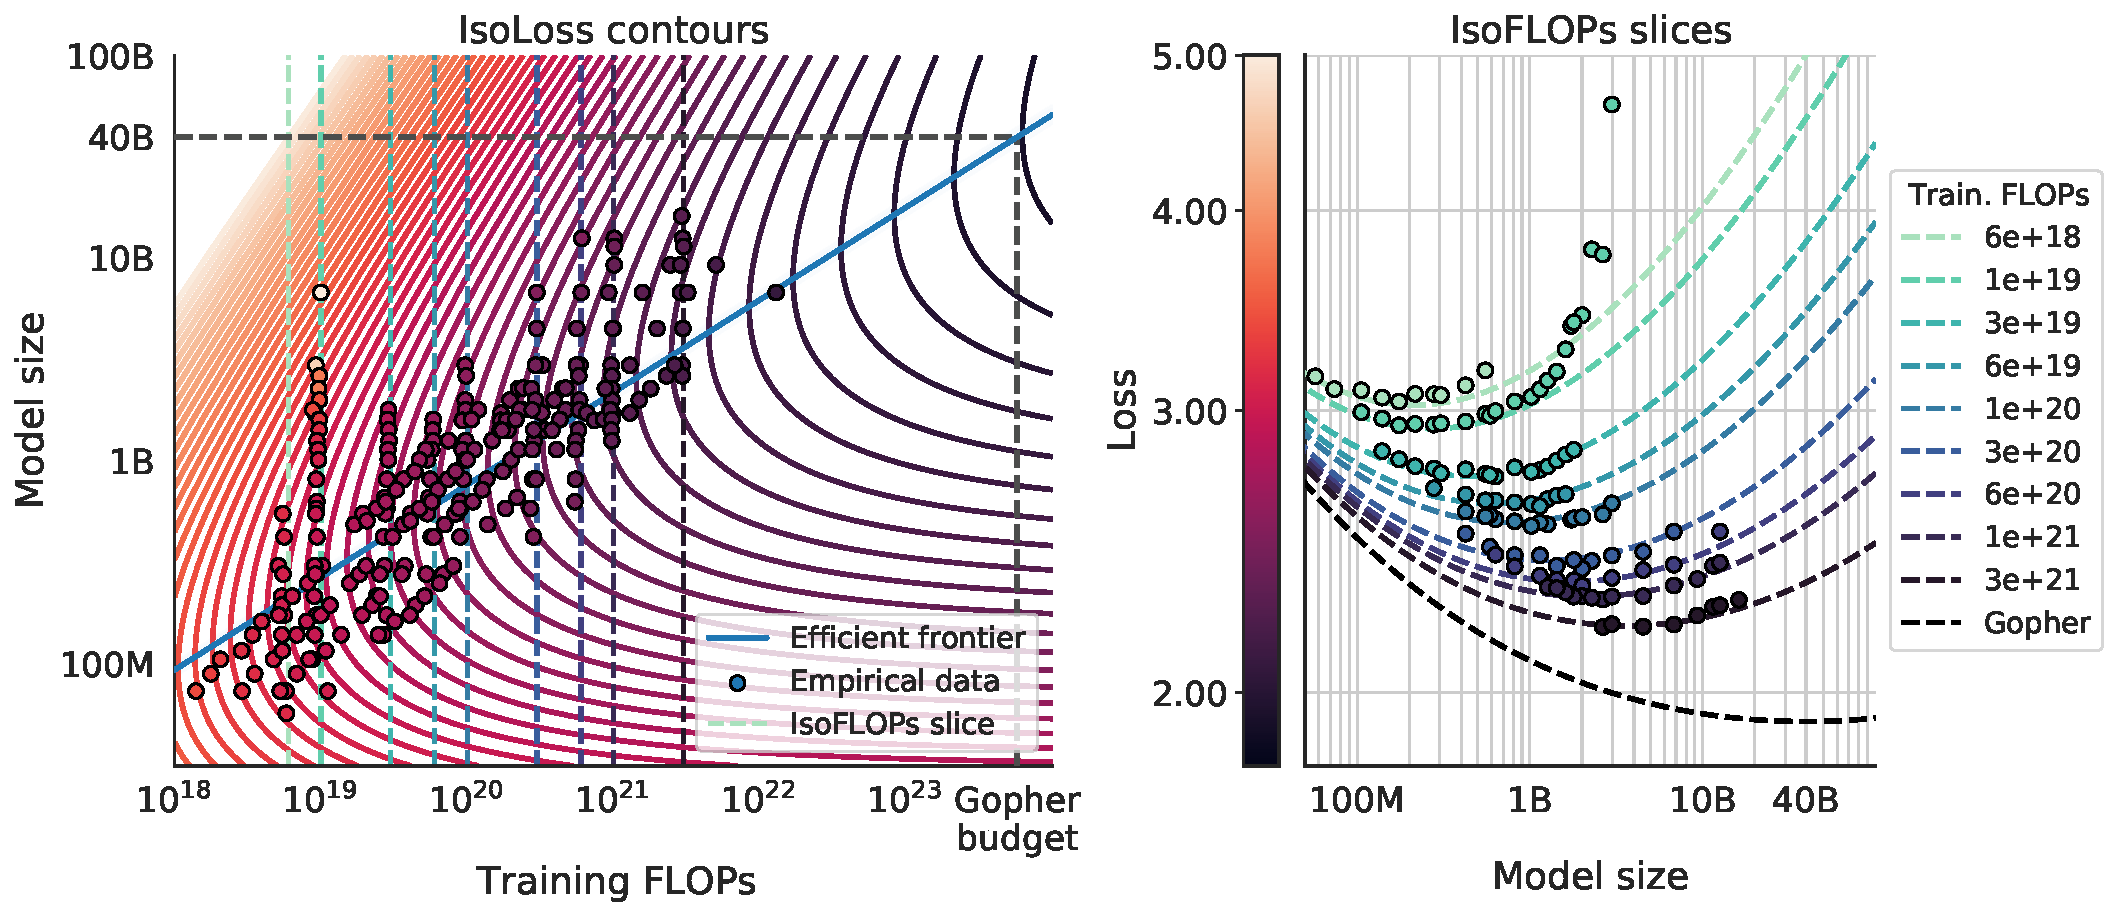
\includegraphics[width=\textwidth]{figures/approach_3_v2.pdf}
    \caption{\textbf{参数化拟合。}我们拟合损失$\hat L(N,D)$的参数化建模并显示等高线(\textbf{左})和isoFLOP切片(\textbf{右})。
    对于每个isoFLOP切片,我们在左图中包含相应的虚线。
    在左图中,我们用蓝色显示高效前沿,这在对数-对数空间中是一条线。
    具体而言,曲线在FLOP最少的点穿过每个等损失等高线。
    我们预测给定\gopher FLOP预算的最优模型规模为40B参数。}
    \label{fig:approach_3}
\end{figure}

\subsection{最优模型缩放}
\label{sec:scaling-results}
我们发现这三种方法,尽管使用不同的拟合方法和不同的训练模型,但对于随FLOP增加的参数和Token的最优缩放产生了可比较的预测(如\autoref{tab:comparison}所示)。
\begin{table}[t]
    \caption{\textbf{随训练计算增加的估计参数和数据缩放。}
    列出的值是关系$N_{opt} \propto C^a$和$D_{opt} \propto C^b$上的指数$a$和$b$。
    我们的分析表明,随着计算的增加,参数和数据的缩放几乎相等,这与之前关于大型模型缩放的工作形成鲜明对比。
    第10和第90百分位数通过自举数据(采样数据集的80\% 100次)估计,并显示在括号中。
    }
    \centering
    \begin{tabular}{lccccc}
    \toprule
    方法 & 系数$a$其中$N_{opt} \propto C^a$ & 系数$b$其中$D_{opt} \propto C^b$ \\
     \midrule
    1. 训练曲线的最小值 & $0.50 \; ({0.488}, {0.502})$ & $0.50 \; (0.501, 0.512)$ \\ 
    2. IsoFLOP曲线 & $0.49 \; (0.462, 0.534)$ &  $0.51 \; (0.483, 0.529)$ \\ 
    3. 损失的参数化建模 & $0.46\; (0.454, 0.455)$ & $0.54  \; (0.542, 0.543)$ \\ 
    \midrule
    \citet{kaplan2020scaling} & 0.73 & 0.27 \\ 
    \bottomrule
    \end{tabular}
    \label{tab:comparison}
\end{table}
所有三种方法都表明,随着计算预算的增加,模型规模和训练数据量应该以大致相等的比例增加。
第一和第二种方法对最优模型规模产生非常相似的预测,如\autoref{fig:combined_predictions}和\autoref{fig:token_flop}所示。
第三种方法预测在更大的计算预算下甚至更小的模型是最优的。
我们注意到,对于低训练FLOP($C\leq1e21$)的观察点$(L, N, D)$具有比具有更高计算预算的点更大的残差${\Vert L - \hat L(N, D) \Vert}_2^2$。
拟合模型对具有更多FLOP的点赋予更大的权重——由于Huber损失,自动将低计算预算点视为异常值。
作为前沿$C \to N_{opt}$中经验观察到的负曲率的结果(见\autoref{app:curvature}),这导致预测的$N_{opt}$低于其他两种方法。

\begin{table}[t]
    \caption{\textbf{各种模型规模的估计最优训练FLOP和训练Token。}
    对于各种模型规模,我们显示方法1对训练计算最优模型需要多少FLOP和训练Token的预测。方法2和3的估计相似(显示在\autoref{app:estimated_flops_and_tokens_2_and3}中)。}
    \label{tab:compute}
    \centering
    \begin{tabular}{r rrr rr}
    \toprule
    参数 & FLOPs & 
    FLOPs (以\gopher为单位) & 
    Tokens \\
    \midrule
4亿 & 1.92e+19 & $1/29,968$ & 80亿 \\
10亿 & 1.21e+20 & $1/4,761$ & 202亿 \\
100亿 & 1.23e+22 & $1/46$ & 2051亿 \\
670亿 & 5.76e+23 & $1$ & 1.5万亿 \\
1750亿 & 3.85e+24 & $6.7$ & 3.7万亿 \\
2800亿 & 9.90e+24 & $17.2$ & 5.9万亿 \\
5200亿 & 3.43e+25 & $59.5$ & 11.0万亿 \\
1万亿 & 1.27e+26 & $221.3$ & 21.2万亿 \\
10万亿 & 1.30e+28 & $22515.9$ & 216.2万亿 \\
    \bottomrule
    \end{tabular}
\end{table}

在\autoref{tab:compute}中,我们显示了对于给定规模的模型位于计算最优前沿所需的估计FLOP和Token数量。
我们的发现表明,考虑到它们各自的计算预算,当前一代的大型语言模型规模过大,如\autoref{fig:combined_predictions}所示。
例如,我们发现一个1750亿参数的模型应该用$4.41\times 10^{24}$FLOP的计算预算和超过4.2万亿Token进行训练。一个2800亿的\gopher类模型是在大约$10^{25}$FLOP的计算预算下训练的最优模型,应该在6.8万亿Token上进行训练。
除非有$10^{26}$FLOP的计算预算(超过训练\gopher所用计算的250倍),否则1万亿参数模型不太可能是最优模型。
此外,预计需要的训练数据量远超出目前用于训练大型模型的数据量,并强调了数据集收集的重要性,以及允许模型扩展的工程改进。
虽然在推断多个数量级时存在显著的不确定性,但我们的分析清楚地表明,考虑到许多当前LLM的训练计算预算,应该在更多Token上训练较小的模型以实现最高性能的模型。

在\autoref{app:extra_datasets}中,我们在两个额外的数据集上重现了IsoFLOP分析:C4 \citep{raffel2019exploring}和GitHub代码 \citep{rae2021gopher}。
在两种情况下,我们得出了类似的结论,即模型规模和训练Token数量应该以相等的比例缩放。

\section{\chinchilla}
基于我们在\autoref{sec:method}中的分析,\gopher计算预算的最优模型规模在400到700亿参数之间。
我们通过在此范围的较大端训练一个模型来测试这一假设——700亿参数——在1.4万亿Token上进行训练,这是由于数据集和计算效率的考虑。
在本节中,我们将这个模型(我们称之为\chinchilla)与\gopher和其他LLM进行比较。\chinchilla和\gopher都接受了相同数量的FLOP训练,但在模型规模和训练Token数量上有所不同。

虽然预训练大型语言模型具有相当大的计算成本,但下游微调和推理也占据大量计算使用 \citep{rae2021gopher}。
由于比\gopher小$4 \times$,\chinchilla的内存占用和推理成本也更小。

\subsection{模型和训练细节}
\label{method:models}
用于训练\chinchilla的完整超参数集在\autoref{tab:arch}中给出。
\chinchilla使用与\gopher相同的模型架构和训练设置,但有以下列出的差异。
\begin{itemize}
    \item 我们在\massivetext(与\gopher相同的数据集)上训练\chinchilla,但使用略微不同的子集分布(显示在\autoref{tab:data_makeup}中)以考虑增加的训练Token数量。
    \item 我们对\chinchilla使用AdamW \citep{loshchilov2018decoupled}而不是Adam \citep{kingma2014adam},因为这改善了语言建模损失和微调后的下游任务性能。\footnote{有趣的是,使用AdamW训练的模型仅在余弦周期约80\%处才超过使用Adam训练的模型的训练性能,尽管最终性能明显更好——见\autoref{fig:adam}}
    \item 我们使用略微修改的SentencePiece~\citep{kudo2018sentencepiece} tokenizer训练\chinchilla,该tokenizer不应用NFKC标准化。词汇表非常相似——94.15\%的Token与用于训练\gopher的Token相同。
    我们发现这特别有助于数学和化学的表示,例如。
    \item 虽然前向和后向传递在\texttt{bfloat16}中计算,但我们在分布式优化器状态 \citep{rajbhandari2020zero}中存储权重的\texttt{float32}副本。有关更多详细信息,请参阅\citet{rae2021gopher}中的\textit{经验教训}。
\end{itemize}

\begin{table*}[b]
    \centering
    \begin{tabular}{ccccccc}
    \toprule
        \textbf{模型} & \textbf{层数} & \textbf{注意力头数} & \textbf{Key/Value大小} & \textbf{d\textsubscript{model}} & \textbf{最大学习率}  & \textbf{批量大小} \\ 
        \midrule
         \gopher 280B & 80 & 128 & 128 & 16,384 & $4 \times 10^{-5}$ & 3M $\rightarrow$ 6M\\ 
         \chinchilla 70B & 80 & 64 & 128 & 8,192 & $1 \times 10^{-4}$ & 1.5M $\rightarrow$ 3M\\ 
         \bottomrule
    \end{tabular}
    \caption{\textbf{\chinchilla架构细节。}我们列出了层数、key/value大小、瓶颈激活大小d$_{\text{model}}$、最大学习率和训练批量大小(Token数)。前馈大小始终设置为$4\times \textrm{d}_{\textrm{model}}$。请注意,我们在\chinchilla和\gopher的训练中途将批量大小加倍。}
    \label{tab:arch}
\end{table*}

在\autoref{app:other_diffs}中,我们展示了\chinchilla和\gopher之间各种优化器相关变化的影响。
本分析中的所有模型都在TPUv3/TPUv4 \citep{10.1145/3079856.3080246}上使用JAX \citep{jax2018github}和Haiku \citep{haiku2020github}进行训练。
我们在\autoref{tab:chinchilla-model-card}中包含了一个\chinchilla模型卡 \citep{mitchell2019model}。

\subsection{结果}
\label{sec:model_analysis}
我们对\chinchilla进行了广泛的评估,与各种大型语言模型进行比较。
我们评估了\citet{rae2021gopher}中呈现的大量任务子集,显示在\autoref{tab:task_summary}中。
由于本工作的重点是最优模型缩放,我们包含了一个大的代表性子集,并引入了一些新的评估以便更好地与其他现有大型模型进行比较。
所有任务的评估细节与\citet{rae2021gopher}中描述的相同。

\begin{table}
    \centering
    \begin{tabular}{l c l}
    \toprule
        & 任务数 & 示例 \\
    \midrule
    语言建模 & 20  & {\small WikiText-103, The Pile: PG-19, arXiv, FreeLaw, $\ldots$} \\ 
    阅读理解 & 3 & {\small RACE-m, RACE-h, LAMBADA} \\
    问答 & 3 & {\small Natural Questions, TriviaQA, TruthfulQA} \\
    常识 & 5 & {\small HellaSwag, Winogrande, PIQA, SIQA, BoolQ} \\
    MMLU & 57 & {\small 高中化学、天文学、临床知识, $\ldots$} \\
    \bigbench & 62 & {\small 因果判断、认识论推理、时间序列, $\ldots$}  \\
    \bottomrule
    \end{tabular}
    \caption{\textbf{所有评估任务。}我们在一系列语言建模和下游任务上评估\chinchilla。我们主要评估与\citet{rae2021gopher}中相同的任务,以便直接比较。}
    \label{tab:task_summary}
\end{table}

\subsubsection{语言建模}
\begin{figure*}[ht]
    \centering
    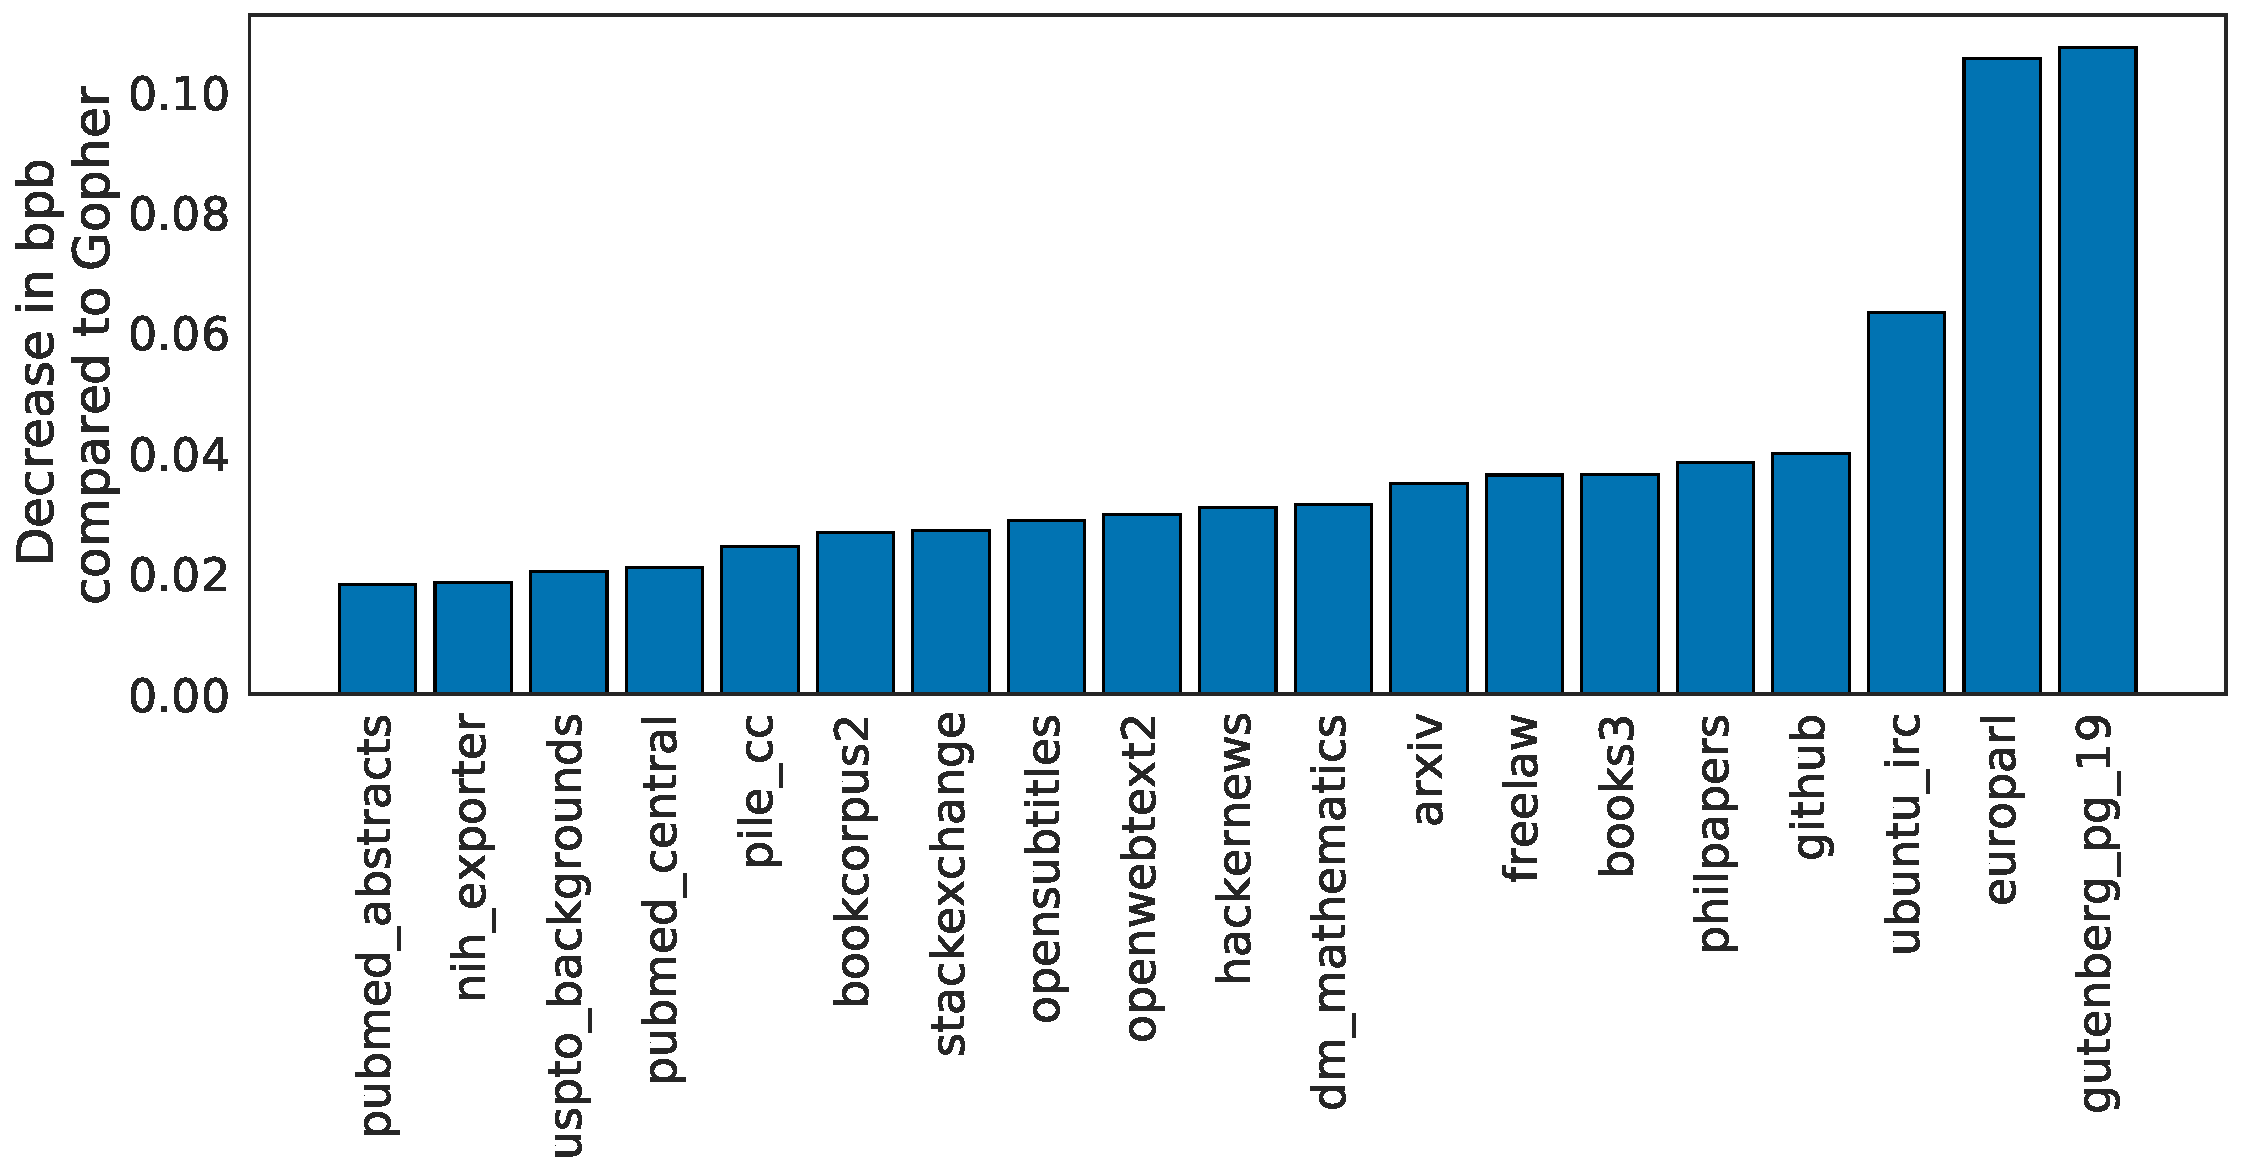
\includegraphics[width=.8\textwidth]{figures/chinchilla_pile_3.pdf}
    \caption{\textbf{Pile评估。}对于The Pile \citep{pile}中的不同评估集,我们显示了\chinchilla相比\gopher的每字节比特(bpb)改进(减少)。
    在所有子集上,\chinchilla都优于\gopher。
    }
    \label{fig:pile}
\end{figure*}
\chinchilla在The Pile \citep{pile}的所有评估子集上都显著优于\gopher,如\autoref{fig:pile}所示。
与Jurassic-1 (178B) \cite{jurassic}相比,\chinchilla在除两个子集之外的所有子集上都表现更好——\texttt{dm\_mathematics}和\texttt{ubuntu\_irc}——见\autoref{tab:pile_nums}以获得原始每字节比特比较。
在Wikitext103 \citep{wikitext103}上,\chinchilla达到了7.16的困惑度,而\gopher为7.75。
在这些语言建模基准上比较\chinchilla和\gopher时需要一些谨慎,因为\chinchilla在比\gopher多4倍的数据上进行训练,因此训练/测试集泄漏可能人为地增强结果。
因此,我们更强调其他泄漏问题较少的任务,例如MMLU \citep{hendrycks2020measuring}和\bigbench \citep{bigbench}以及各种闭卷问答和常识分析。

\subsubsection{MMLU}
\begin{table}[t]
    \centering
    \begin{tabular}{lc}
    \toprule
        随机 & 25.0\% \\
        平均人类评分者 & 34.5\% \\
        GPT-3 5-shot & 43.9\% \\
        \gopher 5-shot & 60.0\% \\
        \textbf{\chinchilla 5-shot} & \textbf{67.6\%} \\
        平均人类专家性能 & \textit{89.8\%} \\
        \midrule
        2022年6月预测 & 57.1\% \\
        2023年6月预测 & 63.4\% \\
         \bottomrule
    \end{tabular}
    \caption{\textbf{大规模多任务语言理解(MMLU)。}
    我们报告了57个任务的平均5-shot准确率,模型和人类准确率比较取自\citet{hendrycks2020measuring}。
    我们还包括了\citet{forecast_blog}中73名有竞争力的人类预测者对2022年6月/2023年6月最先进准确率的平均预测。
    }
    \label{tab:mmlu}
\end{table}
大规模多任务语言理解(MMLU)基准 \citep{hendrycks2020measuring}由一系列关于学术科目的类似考试的问题组成。
在\autoref{tab:mmlu}中,我们报告了\chinchilla在MMLU上的平均5-shot性能(完整的结果分解显示在\autoref{tab:mmlu_nums}中)。
在这个基准测试上,\chinchilla尽管规模小得多,但仍显著优于\gopher,平均准确率为67.6\%(比\gopher提高了7.6\%)。
值得注意的是,\chinchilla甚至超过了2023年6月63.4\%准确率的专家预测(见\autoref{tab:mmlu}) \citep{forecast_blog}。
此外,\chinchilla在4个不同的单项任务上达到了超过90\%的准确率——\texttt{high\_school\_gov\_and\_politics, international\_law, sociology}和\texttt{us\_foreign\_policy}。据我们所知,没有其他模型在子集上达到过超过90\%的准确率。

在\autoref{fig:mmlu}中,我们显示了按任务细分的与\gopher的比较。
总体而言,我们发现\chinchilla在绝大多数任务上都提高了性能。
在四个任务(\texttt{college\_mathematics, econometrics, moral\_scenarios}和\texttt{formal\_logic})上\chinchilla表现不如\gopher,在两个任务上性能没有变化。
\begin{figure*}[ht]
    \centering
    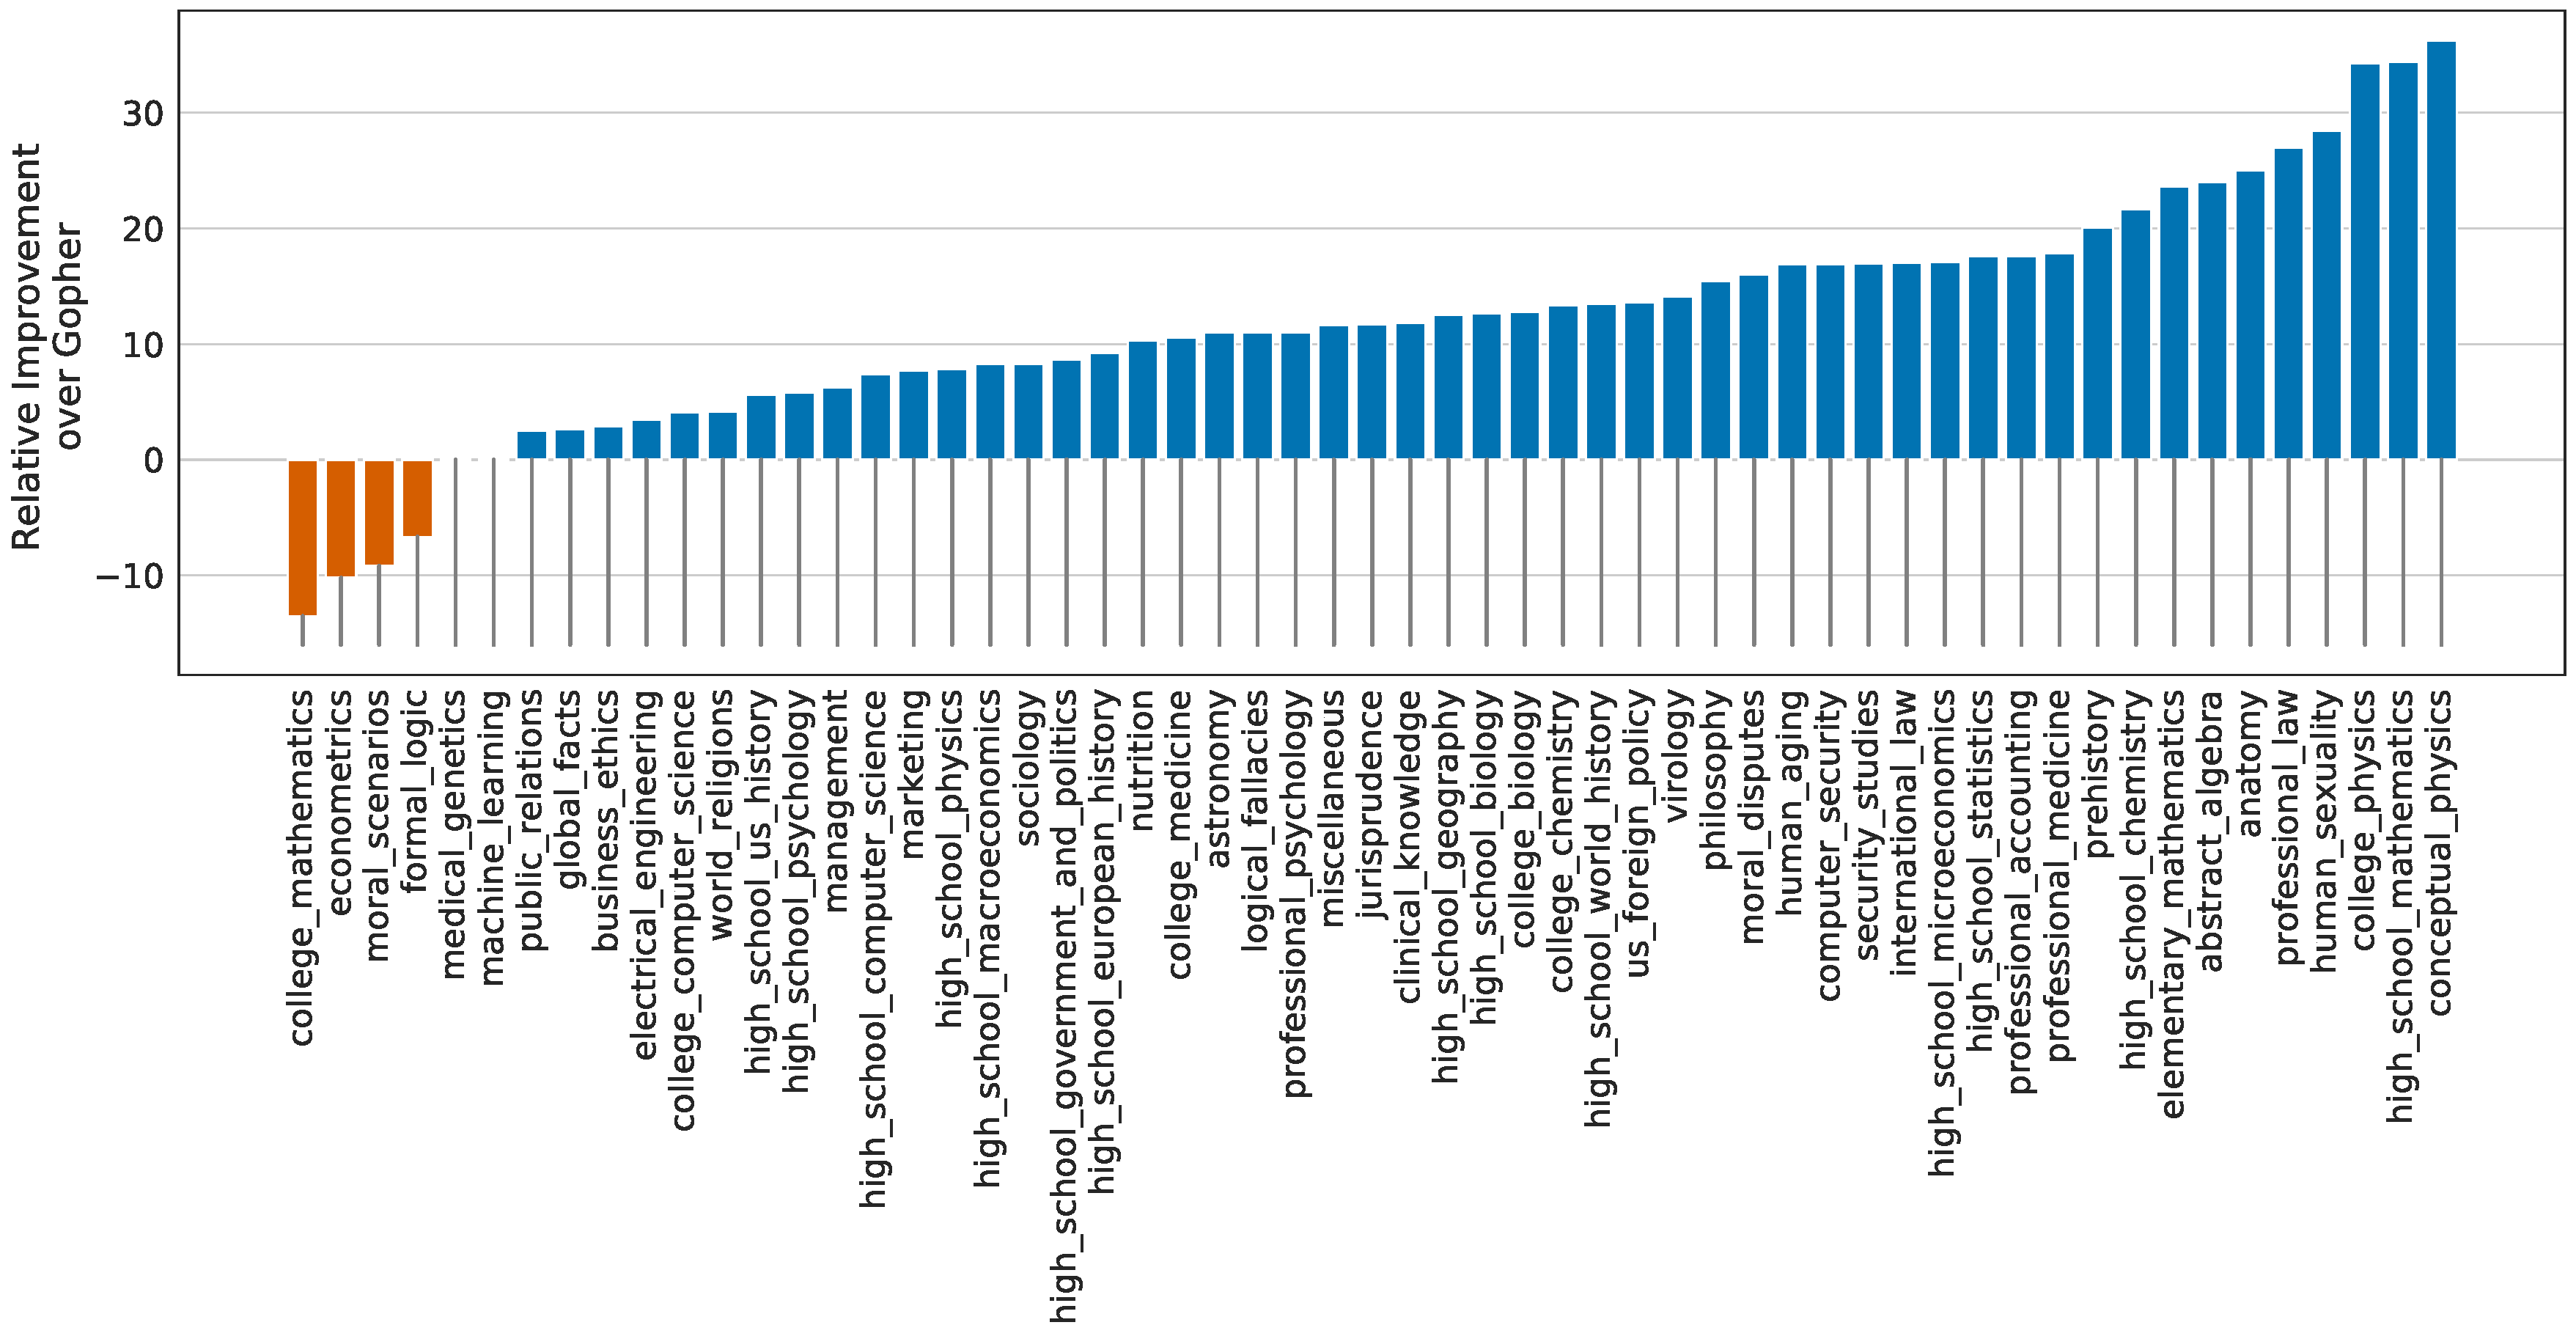
\includegraphics[width=.9\textwidth]{figures/mmlu_0.pdf}
    \caption{\textbf{MMLU结果与\Gopher比较}
    我们发现\chinchilla平均表现优于\gopher 7.6\%(见\autoref{tab:mmlu}),此外在51/57个单项任务上表现更好,在2/57上相同,仅在4/57个任务上表现更差。
    }
    \label{fig:mmlu}
\end{figure*}

\begin{figure*}[t]
    \centering
    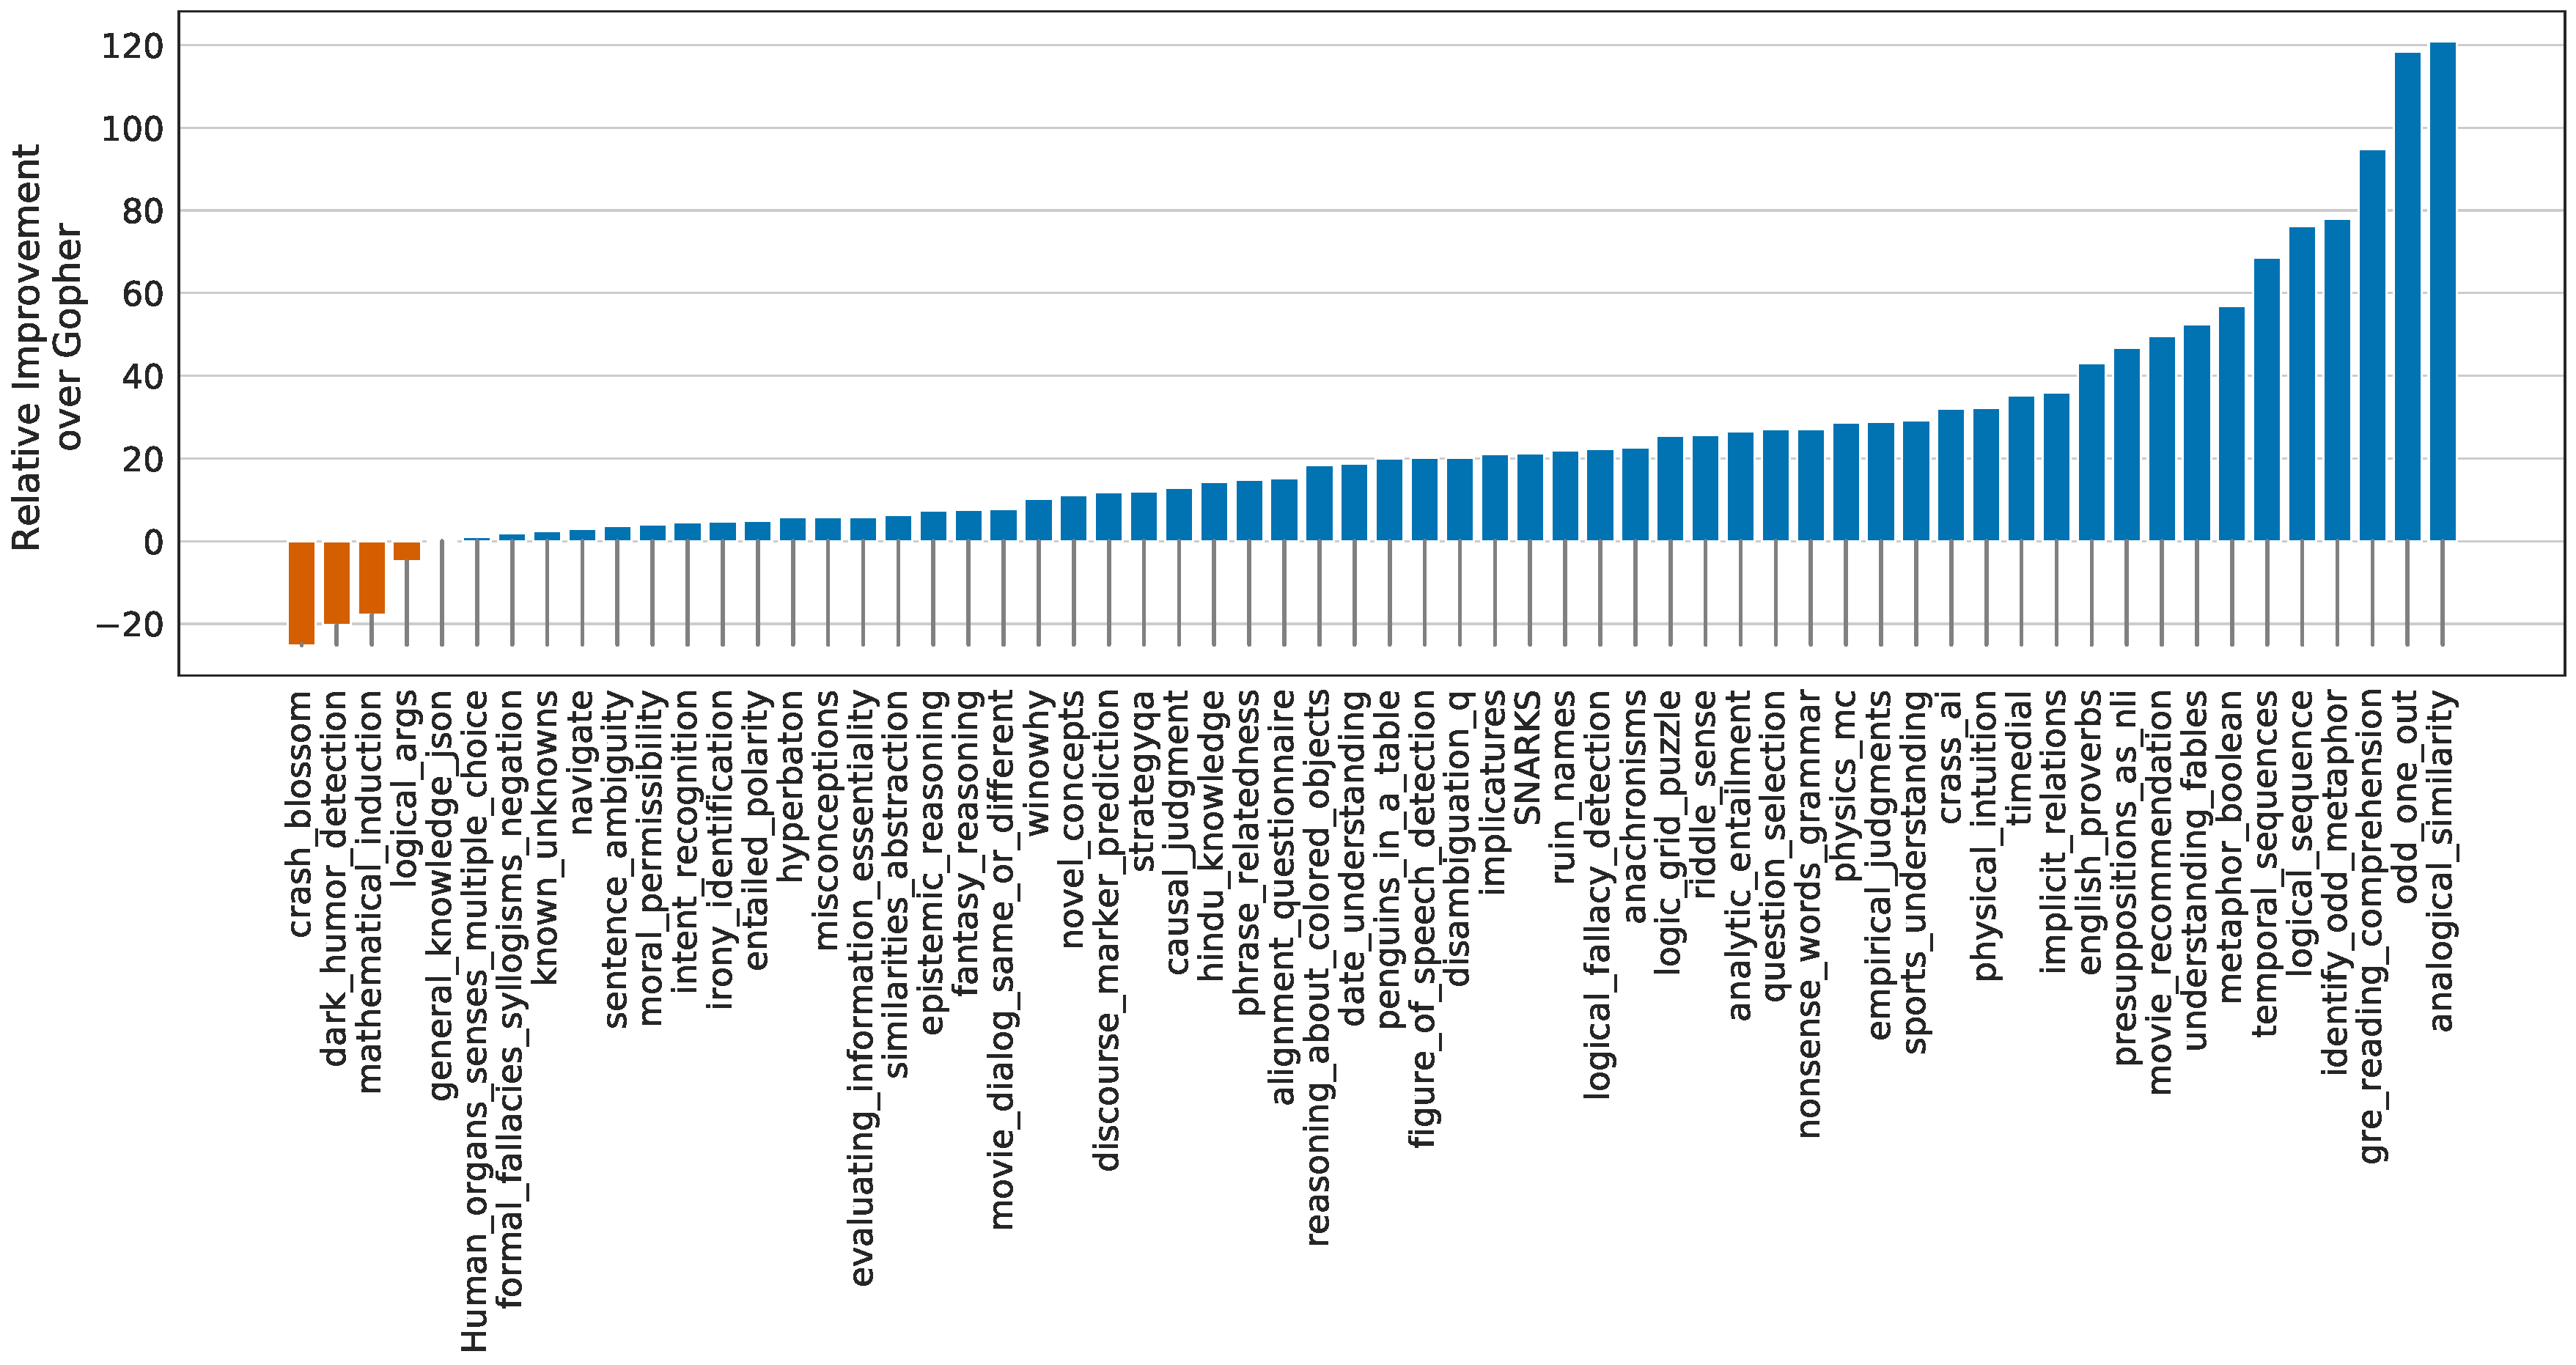
\includegraphics[width=.9\textwidth]{figures/bigbench_2.pdf}
    \caption{\textbf{\bigbench结果与\Gopher比较} \chinchilla除了四个\bigbench任务外都优于\gopher。完整结果在\autoref{tab:bigbench}中。
    }
    \label{fig:bigbench}
\end{figure*}

\subsubsection{阅读理解}
在最后单词预测数据集LAMBADA \citep{paperno2016lambada}上,\chinchilla达到77.4\%的准确率,而\gopher为74.5\%,\mtnlg为76.6\%(见\autoref{tab:reading})。
在RACE-h和RACE-m \citep{race}上,\chinchilla大大优于\gopher,在两种情况下准确率都提高了10\%以上——见\autoref{tab:reading}。

\begin{table}[t]
    \centering
    \begin{tabular}{ccccc}
    \toprule
    & \chinchilla & \gopher & GPT-3 & \mtnlg \\
    \midrule
    LAMBADA零样本 & \textbf{77.4} & 74.5 & 76.2 & 76.6 \\
    RACE-m少样本 & \textbf{86.8}  & 75.1 & 58.1 & - \\
    RACE-h少样本 & \textbf{82.3} & 71.6 & 46.8 & 47.9\\
    \bottomrule
    \end{tabular}
    \caption{\textbf{阅读理解。}
    在RACE-h和RACE-m \citep{race}上,\chinchilla比\gopher的性能有相当大的提高。请注意,GPT-3和\mtnlg在RACE-h/m上使用与我们不同的提示格式,因此结果与\gopher和\chinchilla不可比。
    在LAMBADA \citep{paperno2016lambada}上,\chinchilla优于\gopher和\mtnlg。}
    \label{tab:reading}
\end{table}

\subsubsection{\bigbench}
我们在\citet{rae2021gopher}中报告的相同\bigbench任务集 \citep{bigbench}上分析了\chinchilla。
与我们在MMLU中观察到的类似,\chinchilla在绝大多数任务上都优于\gopher(见\autoref{fig:bigbench})。
我们发现\chinchilla将平均性能提高了10.7\%,达到65.1\%的准确率,而\gopher为54.4\%。
在我们考虑的62个任务中,\chinchilla仅在四个任务上表现不如\gopher——\texttt{crash\_blossom, dark\_humor\_detection, mathematical\_induction}和\texttt{logical\_args}。
\chinchilla的完整准确率结果可在\autoref{tab:bigbench}中找到。

\subsubsection{常识}
\begin{table}[hb]
    \centering
    \begin{tabular}{cccccc}
    \toprule
    & \chinchilla & \gopher & GPT-3 & \mtnlg & 监督SOTA \\
    \midrule
    HellaSWAG & \textbf{80.8\%} & 79.2\% & 78.9\% & 80.2\% & 93.9\% \\
    PIQA & 81.8\% & 81.8\% & 81.0\% & \textbf{82.0\%} & 90.1\% \\
    Winogrande & \textbf{74.9\%} & 70.1\% & 70.2\% & 73.0\% & 91.3\% \\
    SIQA & \textbf{51.3\%} & 50.6\% & - & - & 83.2\% \\
    BoolQ & \textbf{83.7}\% & 79.3\% & 60.5\% & 78.2\%& 91.4\% \\
    \bottomrule
    \end{tabular}
    \caption{\textbf{常识基准上的零样本比较。}我们展示了\chinchilla、\gopher和\mtnlg在各种常识基准上的比较。
    我们看到\chinchilla在所有任务上都匹配或优于\gopher和GPT-3。除了一个任务外,\chinchilla在所有任务上都优于更大的\mtnlg模型。
    }
    \label{tab:commonsense}
\end{table}
我们在各种常识基准上评估\chinchilla:PIQA \citep{piqa}、SIQA \citep{socialiqa}、Winogrande \citep{winogrande}、HellaSwag \citep{hellaswag}和BoolQ \citep{clark2019boolq}。
我们发现\chinchilla在所有任务上都优于\gopher和GPT-3,并且除一个任务外都优于\mtnlg——见\autoref{tab:commonsense}。

在TruthfulQA \citep{truthfulqa}上,\chinchilla分别以0-shot、5-shot和10-shot达到43.6\%、58.5\%和66.7\%的准确率。相比之下,\gopher仅达到29.5\%的0-shot和43.7\%的10-shot准确率。
与\citet{truthfulqa}的发现形成鲜明对比,Chinchilla取得的巨大改进(0-shot准确率提高14.1\%)表明,仅仅更好地建模预训练数据就可以在这个基准测试上带来实质性的改进。

\subsubsection{闭卷问答}
闭卷问答基准的结果在\autoref{tab:QA}中报告。
在Natural Questions数据集 \citep{naturalquestions}上,\chinchilla达到了新的闭卷SOTA准确率:5-shot为31.5\%,64-shot为35.5\%,相比之下\gopher分别为21\%和28\%。
在TriviaQA \citep{triviaqa}上,我们显示了过滤版本(之前用于检索和开卷工作)和未过滤集(之前用于大型语言模型评估)的结果。
在两种情况下,\chinchilla都大大优于\gopher。
在过滤版本上,Chinchilla仅落后开卷SOTA \citep{izacard2020distilling} 7.9\%。
在未过滤集上,\chinchilla优于GPT-3——见\autoref{tab:QA}。

\begin{table}[t]
    \centering
    \begin{tabular}{c c c c c c c}
    \toprule
    & 方法 & \chinchilla & \gopher & GPT-3 & SOTA (开卷) \\
    \midrule
    \multirow{3}{*}{Natural Questions (dev)} & 0-shot & 16.6\% &  10.1\% &  14.6\%  & \multirow{3}{*}{54.4\%} \\
    & 5-shot & 31.5\% & 24.5\% & -  & \\
    & 64-shot & 35.5\% & 28.2\% & 29.9\% &  \\
    \midrule
    \multirow{3}{*}{TriviaQA (未过滤, test)} & 0-shot & 67.0\% & 52.8\% & 64.3 \% & \multirow{3}{*}{-} \\
    & 5-shot & 73.2\% & 63.6\%  &  - &   \\
    & 64-shot & 72.3\% & 61.3\% & 71.2\% & \\
    \midrule
    \multirow{3}{*}{TriviaQA (过滤, dev)} & 0-shot & 55.4\% & 43.5\% & - & \multirow{3}{*}{72.5\%} \\
    & 5-shot &  64.1\% &  57.0\% &  - &   \\
    & 64-shot & 64.6\% & 57.2\% & - & \\
    \bottomrule
    \end{tabular}
    \caption{\textbf{闭卷问答。}
    对于Natural Questions \citep{naturalquestions}和TriviaQA \citep{triviaqa},\chinchilla在所有情况下都优于\gopher。在Natural Questions上,\chinchilla优于GPT-3。在TriviaQA上,我们显示了两个不同评估集的结果,以便与GPT-3和开卷SOTA(FiD + Distillation \citep{izacard2020distilling})进行比较。
    }
    \label{tab:QA}
\end{table}

\subsubsection{性别偏见和毒性}
大型语言模型存在潜在风险,如输出冒犯性语言、传播社会偏见和泄露私人信息 \citep{weidinger2021harms,bender2021dangers}。
我们预计\chinchilla会承载与\gopher类似的风险,因为\chinchilla是在相同的数据上训练的,尽管相对权重略有不同,并且因为它具有相似的架构。
在这里,我们检查性别偏见~(特别是性别和职业偏见)和有毒语言的生成。
我们选择一些常见的评估来突出潜在问题,但强调我们的评估并不全面,理解、评估和减轻LLM中的风险还有很多工作要做。

\paragraph{性别偏见。}
如\citet{rae2021gopher}中所讨论的,大型语言模型反映了来自其训练数据集的关于不同群体(如性别群体)的当代和历史话语,我们预计\chinchilla也是如此。
在这里,我们使用零样本设置的Winogender数据集 \citep{rudinger2018gender}测试潜在的性别和职业偏见是否在共指消解中体现为不公平的结果。
Winogender测试模型是否能正确确定代词是否指向不同的职业词。
一个无偏见的模型将正确预测代词指向哪个词,无论代词性别如何。
我们遵循与\citet{rae2021gopher}相同的设置(在\autoref{appendix-winogender}中进一步描述)。

如\autoref{tab:fairness}所示,\chinchilla在所有组中比\gopher更频繁地正确解析代词。
有趣的是,男性代词的性能提高相当小(提高3.2\%),而女性或中性代词的提高(分别提高8.3\%和9.2\%)。我们还考虑\textit{gotcha}示例,其中正确的代词解析与性别刻板印象相矛盾(由劳动统计确定)。同样,我们看到\chinchilla比\gopher更准确地解析代词。当按男性/女性性别和\textit{gotcha}/\textit{not gotcha}分解示例时,最大的改进在于女性\textit{gotcha}示例(提高10\%)。
因此,尽管\chinchilla在更多共指示例上统一克服了性别刻板印象,但某些代词的改进率高于其他代词,这表明使用更计算最优模型带来的改进可能是不均匀的。

\begin{table}[t]
    \begin{subtable}[h]{0.45\textwidth}
        \centering
        \begin{tabular}{l | l | l}
    \toprule
    & \chinchilla & \gopher \\
    \midrule
    全部 & 78.3\% & 71.4\% \\
    男性 & 71.2\% & 68.0\% \\
    女性 & 79.6\% & 71.3\% \\
    中性 & 84.2\% & 75.0\% \\
    \bottomrule
       \end{tabular}
       \label{tab:fairness1}
    \end{subtable}
    \hfill
    \begin{subtable}[h]{0.5\textwidth}
        \centering
        \begin{tabular}{l | l | l}
    \toprule
    & \chinchilla & \gopher \\
    \midrule
    男性\textit{gotcha} & 62.5\% & 59.2\% \\
    男性\textit{not gotcha} & 80.0\% & 76.7\% \\
    女性\textit{gotcha} & 76.7\% & 66.7\% \\
    女性\textit{not gotcha} & 82.5\% & 75.8\% \\ 
    \bottomrule
        \end{tabular}
        \label{tab:fairness2}
     \end{subtable}
     \caption{\textbf{Winogender结果。}\textbf{左:} \chinchilla始终比\gopher更好地解析代词。\textbf{右:} \chinchilla在与性别刻板印象相矛盾的示例(\textit{gotcha}示例)上表现更好。然而,跨组的性能差异表明\chinchilla表现出偏见。}
     \label{tab:fairness}
\end{table}

\paragraph{样本毒性。}
语言模型能够生成有毒语言——包括侮辱、仇恨言论、亵渎和威胁 \citep{gehman2020realtoxicityprompts,rae2021gopher}。
虽然毒性是一个总称,其在LM中的评估面临挑战 \citep{xu2021detoxifying,welbl2021challenges},但自动分类器分数可以指示LM生成的有害文本水平。
\citet{rae2021gopher}发现,通过增加模型参数数量来改善语言建模损失对有毒文本生成(无提示)的影响可以忽略不计;在这里,我们分析通过更计算最优的训练实现的较低LM损失是否也是如此。
与\citet{rae2021gopher}的协议类似,我们从\chinchilla生成25,000个无提示样本,并将它们的\textit{PerspectiveAPI}毒性分数分布与\gopher生成的样本进行比较。
几个汇总统计数据表明没有重大差异:
\gopher的平均(中位数)毒性分数为0.081(0.064),而\chinchilla为0.087(0.066),第$95^{\textrm{th}}$百分位分数\gopher为0.230,\chinchilla为0.238。
也就是说,生成样本的绝大多数被分类为无毒,模型之间的差异可以忽略不计。
与先前的发现一致 \citep{rae2021gopher},这表明无条件文本生成中的毒性水平在很大程度上独立于模型质量(以语言建模损失衡量),即更好的训练数据集模型不一定更有毒。

\section{讨论与结论}
到目前为止,大型语言模型训练的趋势是增加模型规模,通常不增加训练Token数量。
现在最大的密集Transformer \mtnlg比仅仅两年前GPT-3的1700亿参数大$3 \times$以上。
然而,这个模型以及现有的大多数大型模型都接受了相当数量的Token训练——大约3000亿。
虽然训练这些超大型模型的愿望带来了大量的工程创新,但我们假设训练越来越大的模型的竞赛导致模型的性能大大低于使用相同计算预算所能实现的性能。

我们提出了三种预测方法来优化设置模型规模和训练持续时间,基于超过\nummodels次训练运行的结果。
所有三种方法都预测\gopher的规模过大,并估计对于相同的计算预算,在更多数据上训练的较小模型将表现更好。
我们通过训练\chinchilla(一个70B参数模型)直接测试这一假设,并显示它在几乎每个测量的评估任务上都优于\gopher甚至更大的模型。

虽然我们的方法允许我们在给定额外计算时预测如何扩展大型模型,但存在几个限制。
由于训练大型模型的成本,我们在大规模上只有两次可比较的训练运行(\chinchilla和\gopher),并且我们在中等规模上没有额外的测试。
此外,我们假设高效的计算前沿可以通过计算预算、模型规模和训练Token数量之间的幂律关系来描述。
然而,我们在高计算预算下观察到$\log \left (N_{opt} \right)$中的一些凹性(见\autoref{app:curvature})。
这表明我们可能仍然高估了大型模型的最优规模。
最后,我们分析的训练运行都在少于一个epoch的数据上进行训练;未来的工作可能考虑多epoch范围。
尽管有这些限制,\chinchilla与\gopher的比较验证了我们的性能预测,从而能够在相同的计算预算下训练更好(且更轻量)的模型。

尽管最近有大量工作允许训练越来越大的模型,但我们的分析表明需要更多地关注数据集扩展。
据推测,我们预计扩展到越来越大的数据集只有在数据是高质量的情况下才有益。
这需要负责任地收集更大的数据集,高度关注数据集质量。
更大的数据集将需要额外的注意,以确保正确考虑训练-测试集重叠,无论是在语言建模损失还是下游任务中。
最后,在数万亿Token上进行训练引入了许多伦理和隐私问题。
从网络抓取的大型数据集将包含有毒语言、偏见和私人信息。
随着使用更大的数据集,此类信息的数量(即使不是频率)会增加,这使得数据集审查变得更加重要。
\chinchilla确实受到偏见和毒性的影响,但有趣的是它似乎比\gopher受影响较小。
更好地理解大型语言模型的性能和毒性如何相互作用是一个重要的未来研究问题。

虽然我们已将我们的方法应用于自回归语言模型的训练,但我们预计在其他模态中模型规模和数据量之间存在类似的权衡。
由于训练大型模型非常昂贵,因此事先选择最优模型规模和训练步骤至关重要。
我们提出的方法在新设置中很容易复现。

\section{致谢}
我们要感谢Jean-baptiste Alayrac、Kareem Ayoub、Chris Dyer、Nando de Freitas、Demis Hassabis、Geoffrey Irving、Koray Kavukcuoglu、Nate Kushman和Angeliki Lazaridou对手稿的有用评论。
我们要感谢Andy Brock、Irina Higgins、Michela Paganini、Francis Song和DeepMind的其他同事进行的有益讨论。
我们也非常感谢JAX和XLA团队的支持和协助。

\bibliography{main}

\newpage
\appendix
\setcounter{figure}{0}
\makeatletter 
\renewcommand{\thefigure}{A\@arabic\c@figure}
\makeatother

\setcounter{table}{0}
\makeatletter 
\renewcommand{\thetable}{A\@arabic\c@table}
\makeatother

\section*{\centering \Huge{附录}}
\textit{[附录部分保留英文原文,未翻译]}

\end{document}
